\chapter{基于多模态的缺陷检测}

\section{多模态缺陷检测框架}
3D数据在检测结构缺陷上具有优势,而RGB图像对于纹理缺陷则更有优势。当面对可能同时具有结构和纹理缺陷的场景,综合利用3D数据和RGB图像能够取得更好的效果。其中由于RGB数据的表现形式是二维图像,因此本文选择使用同样为二维图像的深度图作为3D数据与RGB数据融合作为输入,从而实现多模态的缺陷检测算法。

本文采用异构教师学生网络(AST)\cite{rudolphAsymmetricStudentTeacherNetworks2022}作为多模态缺陷检测的骨干网络。AST目标是训练两个异构的模型,一个记作学生模型$f_{s}$,另一个一个记作教师模型$f_{t}$。其中学生只根据无缺陷的正常样本来回归教师网络的输出,其假设在正常样本上训练的教师学生网络在缺陷样本上有较大差异。整个训练过程分为两个阶段:

首先是训练教师网络模型,本文利用标准化流将训练数据分布$p_{X}$通过双射变换函数转换为正态分布N(0,I)。然后,通过最小化训练样本 $x \in X$的 $f_{s}(x)$和$f_{t}(x)$之间的距离,优化学生网络来匹配教师网络的输出。最后,在测试网络性能时,利用教师学生之间的距离计算异常评分。

本文不直接将RGB图像输入骨干网络,而是利用在ImageNet上预训练的网络模型作为通用特征提取器,对图像进行特征提取后再输入。对于深度图像,本文引入HOG特征描述子来进行深度特征提取,其特征维度与RGB的特征图相匹配,从而方便后续融合。在提取特征前,本文利用多模态的优势,通过深度图像的前景提取来创建蒙版,并用于RGB图像前景提取和后续的距离损失计算,相比于单独使用RGB图像,有效降低了计算量并且提升了性能。
\begin{figure}[htbp]
    \centering
    \includegraphics[width=1\textwidth]{figures/4/framework.pdf}
    \caption{多模态缺陷检测框架}
    \label{fig:4-framework}
\end{figure}

此外,为应对与位置相关的缺陷,本文还采用位置编码的方法来对输入特征图的进行位置编码,并用于学生和教师网络。本文的多模态缺陷检测整体框架如图\ref{fig:4-framework}所示



\section{多模态输入预处理}
\subsection{RGB和深度图像对齐}
RGB 图像在深度学习中被广泛用于各种任务。RGB 图像具有红色(R)、绿色(G)和蓝色(B)三个通道,每种通道都有一个从 0 到 255 的值,其中 0 表示没有颜色,255 表示全色。通过这三个通道可以表示图像的不同特征。不过RGB 图像在计算机视觉任务中也有一些局限性。例如,RGB 图像对光照变化、遮挡和阴影很敏感。 RGB 图像也可能无法区分具有相似颜色或形状的对象。

为了克服这些挑战,在视觉任务的实际应用中,一些方法会在RGB图像的基础上在引入更直观表现深度信息的深度图像,组合成RGB-D 图像。由于深度测量相机可以直接计算与图像中每个像素之间的距离,与单独使用 RGB 图像相比,RGB-D 图像可以为物体检测提供更丰富、更稳健的特征。因此 RGB-D 图像可以比 RGB 图像更好地处理遮挡、阴影和复杂背景。

通常来说,深度信息和RGB信息由于采集方式的不同,深度图和RGB图之间的坐标系往往也不同,这会对下游分类检测等任务产生影响。因此想要综合利用深度图和RGB图的信息就需要将两者进行坐标变换,必须将深度图和RGB图的坐标对齐。常用的对齐深度图和RGB图的方法包括通过相机本身的内外参进行对齐和通过关键点或特征匹配来实现对齐,其中采用相机内外参的方式进行对齐更加简单稳定。

针对本文使用的结构光相机,RGB摄像头的成像平面坐标系作为基准坐标系,以RGB摄像头光心位置为坐标原点,遵循右手定则。首先按照第二章讨论的相机模型的坐标系之间的关系获取 RGB-D 相机的 RGB 摄像头的内参矩阵、深度摄像头的内参矩阵和RGB 摄像头与深度摄像头的外参旋转矩阵和偏移矩阵,然后遍历深度图像中的每一个像素点坐标,通过如下公式,计算深度图像中像素点对应 RGB 图像中的像素点的坐标。

$$
\left[\begin{array}{l}
X_{d}  \\
Y_{d} \\
Z_{d}
\end{array}\right]=Z_{d}\left[\begin{array}{ccc}
f_{dx} & 0 & u_{d} \\
0 & f_{dy} & v_{d}\\
0 & 0 & 1
\end{array}\right]^{-1}\left[\begin{array}{c}
j_{d} \\
i_{d} \\
1
\end{array}\right]\\
$$

$$
\left[\begin{array}{l}X_{r g b} \\Y_{r g b} \\Z_{r g b}\end{array}\right]=R_{3 \times 3}\left[\begin{array}{l}X_{\text {d }} \\Y_{\text {d}} \\Z_{\text {d}}\end{array}\right]+T_{3 \times 1}
$$

$$
\left[\begin{array}{l}i_{rgb}  \\j_{rgb} \\1\end{array}\right]=\left[\begin{array}{ccc}f_{rgbx} & 0 & u_{rgb} \\0 & f_{rgby} & v_{rgb}\\0 & 0 & 1\end{array}\right]\left[\begin{array}{c}X_{rgb} \\Y_{rgb} \\Z_{rgb}\end{array}\right]/Z_{rgb}
$$

其中,R是RGB摄像头与深度摄像头的外参旋转矩阵, T是偏移矩阵。相机内参矩阵中u,v为光学中心,f表示焦距。X、Y和Z表示空间中的点,i和j表示二维图像中像素位置,下标d和rgb分别表示所属空间坐标系。

\subsection{融合前景提取}
融合前景提取是指综合利用多模态输入,将感兴趣的前景提取出来用于下游任务的处理。通过融合前景提取可以去除背景噪声,提高识别精度。由于提取的前景专注于特定区域而不是整个图像,从来降低了图像处理的计算复杂度和存储空间。此外,当整个图像各局部差别较大,而图像处理方法(例如直方图均衡、自适应阈值等)应用于整个图像效果不佳时,通过提取前景能够是图像处理方法更加灵敏。

通常针对RGB图像,前景提取是通过人工观察图像,手动给出ROI区域,例如通过给定矩形四个顶点在图像坐标系下的坐标值来进行选择。而拍摄物体的几何形状一般较为复杂,简单的手工几何形状难以将背景噪声去除,但如果采用手工逐点标注,效率低且成本高,不符合工业化要求。一些研究通过使用目标检测和分割的网络实现提取拍摄物体ROI,这种方法相对于人工有更高的效率,但对标注数据有一定要求。

本文将RGB图像和深度图像对齐后,RGB图像的每个像素都对应深度图的像素(即每个像素都有一个深度值)。通过综合手工设定区域粗提取,再配合深度图形的深度信息细提取,可以既简单又高效地将拍摄物体与背景进行分离。提取前景后,为保证图像符合输入尺寸,本文将输入图像空间内,前景区域外的空白像素的RGB值设置为(0,0,0),深度值也设置为0。

\section{RGB图像特征提取}
\subsection{卷积神经网络}
卷积神经网络(Convolutional Neural Network,CNN)广泛应用于计算机视觉任务中,其核心思想是通过卷积操作从原始数据中提取特征,再通过池化、非线性激活函数等方式对特征进行处理,最终实现对输入数据的分类或识别。

CNN的主要组成部分包括卷积层和池化层。

\subsubsection{卷积层}

卷积层(Convolutional Layer)是卷积神经网络的核心组件之一,主要用于从图像中提取特征。卷积层采用滤波器(Filter)或卷积核(Kernel)对输入数据进行卷积操作,将输入数据转换为一组特征图(Feature Map),并保留输入数据的局部特征和空间结构。

卷积操作可以看作是一种特殊的线性操作,将输入数据中的每一个小区域与卷积核进行点乘和求和,得到一个特征值。通过移动卷积核,可以在整个输入数据上进行滑动卷积操作,得到一组特征图。在卷积操作中,卷积核的大小、步幅(Stride)和填充(Padding)等参数可以影响特征图的大小和数量,从而影响模型的性能。

卷积层的主要优势在于可以提取输入数据的局部特征和空间结构,具有很好的平移不变性(Translation Invariance)和局部连接性(Local Connectivity)。同时,卷积层的参数共享和稀疏连接性(Sparse Connectivity)可以大幅减少模型的参数数量和计算复杂度,提高模型的训练和推理效率。

在卷积神经网络中,通常会使用多层卷积层来提取多层次的特征表示。随着深度的增加,卷积层的感受野(Receptive Field)也会逐渐增大,可以学习到更高层次的特征表示。

\subsubsection{池化层}

池化层(Pooling Layer)是卷积神经网络的另一个核心组件,主要用于减少特征图的尺寸和数量,提高模型的计算效率和泛化能力。池化层可以通过对特征图进行下采样(Subsampling)或平均池化(Average Pooling)等操作,将特征图的维度缩小,同时保留输入数据的部分特征。

池化操作通常可以看作是一种非线性降采样操作,通过对输入数据中的局部区域进行池化操作,将区域内的信息压缩为一个特征值。常见的池化操作包括最大池化(Max Pooling)、平均池化(Average Pooling)和L2范数池化(L2-Norm Pooling)等,其中最大池化是最常用的一种池化操作。在最大池化中,对于每个池化区域,选择其中的最大值作为该区域的池化结果,从而提取出局部的最强特征。

池化层的主要优点在于可以减少特征图的尺寸和数量,同时保留输入数据的部分特征。通过缩小特征图的尺寸,池化层可以减少模型的参数数量和计算复杂度,提高模型的训练和推理效率。同时,池化层也具有一定的平移不变性和部分不变性,可以对输入数据的轻微变形和平移等变化具有一定的鲁棒性。

在卷积神经网络中,通常会在多层卷积层之间插入池化层,以便逐渐减少特征图的尺寸和数量,同时提取多层次的特征表示。在池化层的设计中,常常需要考虑池化区域的大小、步幅和填充等参数,以及不同池化操作的优缺点,从而平衡模型的性能和计算效率。

此外,卷积层和池化层也可以与其他组件(如批归一化层、非线性激活函数等)结合使用,构建出更加强大的卷积神经网络模型。

CNN的训练主要使用反向传播算法进行优化,可以通过损失函数来度量模型的性能,通过梯度下降法来更新模型参数。在训练过程中,CNN可以通过dropout、批归一化等方式来缓解过拟合问题,提高模型的泛化能力。

\subsection{EffcientNet}
EfficientNet\cite{tanEfficientNetRethinkingModel}是由Google Brain团队提出的一种高效的卷积神经网络(CNN)结构,其通过在卷积层、池化层和全连接层等不同层次上对模型进行深度、宽度和分辨率的统一缩放,实现了在模型参数数量和计算复杂度双重限制下的最优模型结构。与传统的卷积神经网络相比,EfficientNet在参数量和计算复杂度方面都具有更好的性能。同时,在保持准确率的同时,EfficientNet可以显著减少模型的尺寸和计算量,可以有效地提高模型的训练和推理效率。

EfficientNet的核心思想是基于模型缩放(Model Scaling),通过在模型深度、宽度和分辨率等不同维度上进行统一的缩放操作,实现了模型结构的最优化。

在模型深度方面,EfficientNet使用了一种复合系数(Compound Scaling)的方法,同时缩放卷积层的深度和宽度,以保持模型的有效性和可训练性。

在模型宽度方面,EfficientNet采用了一种特殊的宽度因子(Width Multiplier),通过调整每层卷积层的输出通道数,以适应不同的任务需求和计算资源限制。

在模型分辨率方面,EfficientNet则使用了一种新颖的图像增强策略(AutoAugment),通过对输入图像进行多样化的随机增强,提高了模型的数据多样性和泛化能力。

通过综合考虑这三个方面的因素,EfficientNet可以在保持准确率的前提下,同时实现高效的训练和推理。

具体地说,EfficientNet的网络结构由多个卷积层和池化层组成,其中包括一系列的MBConv块(Mobile Inverted Residual Bottleneck Blocks),这些块包含了多个卷积和池化操作,并采用了一种特殊的残差连接方式,以提高模型的非线性表示能力和泛化能力。

在模型结构的缩放过程中,EfficientNet通过一个复合系数φ来平衡模型深度、宽度和分辨率等维度的缩放比例,具体地,模型的宽度、深度和分辨率可以表示为:
$$
\left\{\begin{matrix}
 d=\alpha^{\phi}\\
 w=\beta^{\phi}\\
r=\gamma^{\phi}
\end{matrix}\right.
$$

其中,$\alpha$、$\beta$和$\gamma$分别为宽度、深度和分辨率的缩放系数,$\phi$为复合系数,$w$、$d$和$r$分别表示模型的宽度、深度和分辨率。

EfficientNet在各种计算机视觉任务中都取得了很好的表现,证明了其强大的特征提取能力。此外,EfficientNet还具有良好的迁移性,可以通过微调等方式应用于各种计算机视觉任务中。

\subsection{预训练}
对于本文所研究的工业缺陷检测这类样本难以获取的少样本视觉检测任务来说,无法提供足量数据来训练大型网络是目前主要问题。

预训练是一种在使神经网络模型适应特定任务之前在大量数据上训练神经网络模型的技术。因为预训练的模型已经学习到了一些通用的视觉特征,这些特征可以在其他视觉任务中重复使用。因此使用预训练的网络作为特征提取器允许使用比原始数据集小得多的数据来训练一个有用的模型。对于本文的无监督缺陷检测任务,这是非常重要的特性。

在上一小节介绍到EfficientNet 是一系列卷积神经网络,可以根据任务不同的资源选择合适的变体。EfficientNet 的变体具有不同的复合系数,范围从 0 到 7。系数越高,模型越大越准确,但计算量也越大。

EfficientNet-B5 是变体之一,复合系数为 5,这意味着它具有比其他变体更大的深度、宽度和分辨率。 EfficientNet-B5 有 30M 参数,7.1B FLOPS,其在ImageNet上的表现亮眼。ImageNet是一个大规模的图像识别数据库,由斯坦福大学的研究人员于2009年创建。该数据库包含超过1400万张高质量人工标注图像,常被作为预训练图像分类模型的数据库。

Rudolph等\cite{rudolphAsymmetricStudentTeacherNetworks2022}使用在ImageNet上预训练的EfficientNet-B5,并将其第36层输出特征图作为下游缺陷检测任务的输入,实验结果证明其能很好平衡缺陷检测对特征语义和空间分辨率的需求。

本文被测物的尺寸大小与其接近,因此选择预训练的EfficientNet-B5的36层作为特征提取器。特征提取器的参数只在ImageNet上预训练时调整,在后续缺陷检测任务中,特征提取器参数将保持不变。因此,输入预训练特征提取器的图像需要重新调整尺寸来适配特征提取器的输入维度,即调整为 $768 \times 768$ 分辨率的图像。特征提取器的输出为$24 \times 24$尺寸,304个通道的特征图。

\section{深度图像特征提取}
HOG(Histogram of Oriented Gradients)是一种广泛应用于计算机视觉领域的特征描述子,主要用于目标检测、识别和分类任务。HOG的基本思想是利用图像局部区域的梯度方向和幅值信息来描述图像的形状和纹理特征。其主要特点是对图像的光照和尺度变化具有较强的鲁棒性。

简单来说,HOG首先对输入图像进行归一化处理,消除光照对特征提取的影响;然后计算图像中每个像素点的梯度幅值和方向;接着将图像划分为若干单元格,并在每个单元格内创建梯度方向直方图;之后对直方图进行归一化处理,以消除光照的影响;最后将所有归一化直方图拼接成一个特征向量,即HOG描述子。

HOG最初由Dalal和Triggs提出\cite{dalalHistogramsOrientedGradients2005},主要是针对RGB图像进行特征提取的,但它也可以扩展到提取深度图像特征中。在深度图像中,HOG算法可以用来提取物体的表面纹理、形状等特征,为下游任务提供输入。

深度图像HOG描述子的计算过程包括预处理、梯度计算、梯度方向直方图计算以及特征向量拼接,其中梯度方向直方图计算又包括单元格划分、直方图创建以及归一化。整体流程如算法所示,下文对主要步骤进行简介。

\subsection{预处理}

对于RGB图像,其每个通道的像素值表示通道对应颜色的亮度,在固定的区间内,即[0,255],可以通过将RGB图像转换为灰度图像来应用HOG。而深度图像只有一个通道,每个像素值表示距离摄像头的距离,其值由拍摄时的实际情况决定,并没有明确范围。

因此计算深度图像的HOG就需要对其进行预处理,常见的方法是是将深度图像进行归一化处理,目的是将像素值(距离或深度信息)缩放到一个统一的范围,以消除数据中的尺度差异和减少噪声的影响。归一化预处理流程如下:

(1)将深度图像转换为浮点数格式。为了避免在计算过程中发生整数溢出或损失精度,首先将深度图像转换为浮点数格式,例如float32或float64。

(2)去除无效值。在某些深度图像中,可能存在无效的像素值(例如NaN或负数),这些值表示距离测量失败或不准确。在归一化之前,可以将这些无效值替换为零或其他有效值。

(3)计算最小值和最大值。遍历深度图像,找到有效像素值的最小值$D_{min}$和最大值$D_{max}$。这些值将用于确定缩放因子。

(4)归一化:使用以下公式将每个像素值缩放到指定范围(如0到1):
$$
P_{n} = \frac{P_{o} - D_{min} }{D_{max}-D_{min}}
$$

其中$P_{n}$是归一化后的像素值,$P_{o}$是原始像素值。这个公式将原始像素值线性地映射到0-1范围内,使得最小值对应0,最大值对应1。此外也可以选择其他归一化范围,例如-1到1。

在归一化处理后,对噪声影响成像的情况,可以通过对深度图像应用平滑滤波器(如高斯滤波器或中值滤波器)来去除噪声,提高特征提取的准确性和鲁棒性。

\subsection{梯度计算}

在计算HOG描述子时,算法需要获得图像中每个像素的梯度幅值(magnitude)和梯度方向(orientation)。为了实现这一点,通常使用差分滤波器(Difference Filters)或卷积操作来计算图像的梯度。常用的差分滤波器有Sobel算子、Prewitt算子和Scharr算子。本文通过在水平方向和垂直方向上应用Sobel算子来计算深度图像梯度,不同于RGB图像,深度图像的梯度表示的是空间结构的变化,而非亮度变化。

Sobel算子是一对$3 \times 3$的卷积核,分别用于计算水平梯度$S_{x}$和垂直梯度$S_{y}$,如式\ref{equ:sobel}所示
\begin{equation}\label{equ:sobel}
S_x=\left[\begin{array}{ccc}
-1 & 0 & 1 \\
-2 & 0 & 2 \\
-1 & 0 & 1
\end{array}\right], S_y=\left[\begin{array}{ccc}
-1 & -2 & -1 \\
0 & 0 & 0 \\
1 & 2 & 1
\end{array}\right]
\end{equation}

将这两个卷积核分别逐像素与原图像$M$做卷积运算,得到水平梯度图$G_{x}$和垂直梯度图$G_{y}$,如式\ref{equ:gx} 所示:
\begin{equation}\label{equ:gx}
	G_x = S_x * M, G_y = S_y * M
\end{equation}

接下来,需要结合两张梯度图计算对应每个像素的梯度幅值和梯度方向。其中梯度幅值$|G|$可以通过式\ref{equ:magnitude}计算:
\begin{equation}\label{equ:magnitude}
|G|  = \sqrt{G_x^2 + G_y^2}
\end{equation}

梯度方向$\theta$可以通过式\ref{equ:orientation}计算:
\begin{equation}\label{equ:orientation}
	\theta = \arctan \left ( \frac{G_y}{G_x} \right ) 
\end{equation}


上述梯度方向的计算结果通常是弧度制,可以将其转换为角度制$(0^{\circ} \sim 360^{\circ})$以便于创建方向梯度直方图。

\subsection{梯度方向直方图计算}
获得深度图像每个像素梯度方向和梯度幅值后就可以开始进行直方图统计,具体步骤如下:

(1)分割单元格。将深度图像分割成小的矩形区域,称为单元格(cell)。每个单元格通常包含若干个像素(例如,8x8或16x16像素)。

(2)创建直方图。在每个单元格内,根据梯度方向和幅值,创建一个方向梯度直方图。直方图的每个区间(bin)代表一个特定的梯度方向范围(例如,$0^{\circ} \sim 20^{\circ}$、$20^{\circ} \sim 40^{\circ}$等),区间的值为该方向范围内所有像素梯度幅值的累加。如此,每个单元格都可以用一个梯度方向直方图来描述。

此外,在深度图像中,物体表面的形状和纹理信息比RGB图像更为丰富,因此可以使用更多的方向区间(bin)和更大的单元格尺寸来提高特征的表达能力。

(3)块内直方图归一化。为了消除光照对特征描述子的影响,需要对直方图进行归一化。这通常是通过将每个单元格与其相邻的单元格(例如2x2个单元格)组合成一个较大的区域(称为“块”)。块可以重叠,以确保每个单元格都被归一化。相较一般的RGB图像,在深度图像中,块也可以选择更大尺寸。

对于每个块,可以通过计算块内所有单元格梯度直方图的平方和,即L2范数,然后将每个直方图除以该平方和的平方根来实现将包含的单元格的梯度方向直方图归一化。这个过程可以表示为:
\begin{equation}
	\mathrm{B}=\frac{v}{\sqrt{\|v\|_2^2+\epsilon^2}}
\end{equation}

其中$\mathrm{B}$是块内归一化的直方图,$v$是原始直方图,$\epsilon$表示很小的常数。


\subsection{特征向量拼接}
最后,将前述步骤里所有块内的归一化直方图拼接成一个特征向量,即为本文所需的用于深度图像的HOG描述子,这个特征向量捕捉了深度图像中物体表面的空间变化和局部形状特征,可用于本文下游的缺陷检测任务。特征向量拼接如式所示
\begin{equation}
	\mathrm{HOG}=\left [\mathrm{B}_{1}, \mathrm{B}_{2}, \cdots, \mathrm{B}_{l}\right ]
\end{equation}
其中$l$是块的数量。每个块$\mathrm{B}$的维数为块内单元格数量$c$和每个单元格内区间数量$n$的乘积,因此HOG每个块的维数dims为
\begin{equation}
	\operatorname{dims}=\mathrm{c} \times \mathrm{n}
\end{equation}



\section{教师网络}
本文的教师网络使用标准化流(Normalizing Flow),其是一种具有可追踪分布的生成模型,其原理是利用一系列可逆且可导的函数变换(比如仿射变换)来建模复杂的概率分布,从而实现将简单、已知的分布(例如标准正态分布)转换成目标分布。

标准化流由Rezende和Mohamed\cite{rezendeVariationalInferenceNormalizing2016}在变分推理的背景下推广,由Dinh等人\cite{dinhDensityEstimationUsing2017,lelanPerfectDensityModels2021}用于密度估计。变量替换公式是标准化流通过选择初始概率密度然后经过一系列参数化的可逆可微的变换来构建新分布机制的理论基础。定理\ref{them:varible}介绍了变量替换公式的具体内容。

\begin{them}[变量替换公式]\label{them:varible}
设$X$是一个概率密度函数为 $f_{X}$的连续型随机变量,并设存在一个区间 $I \subset \mathbb{R}$使得当$x \notin I$时,$f_{X}(x)=0$(换句话说,$X$只有在$I$中取值时,其概率密度函数才可能不为0,其中$I$可以是整个实直线).设$g: I \rightarrow \mathbb{R}$是一个可微函数,其反函数是$h$。除了在有限多个点处的导数值可能为0外,$g$的导数在$I$中始终为正或者始终为负.如果令$Y=g(X)$,那么
$$
f_{Y}(y)=f_{X}(h(y)) \cdot\left|h^{\prime}(y)\right| .
$$
\end{them}

根据定理\ref{them:varible},样本的概率密度估计可以通过将它逆变换到原始简单分布,然后计算逆变换样本的概率密度和逆变换序列引起的体积变化间的乘积。这里所说的体积变换实际上就是计算出每个变换相应雅可比矩阵的行列式绝对值再连乘求积。\cite{kobyzevNormalizingFlowsIntroduction2021}

定义 $\mathbf{Z} \in \mathbb{R}^{D}$ 是一个随机变量,其概率密度函数定义为 $p_{\mathbf{Z}}: \mathbb{R}^{D} \rightarrow \mathbb{R}$ 。定义g 是一个可逆函数,并且 $\mathbf{Y}=\mathbf{g}(\mathbf{Z})$。然后通过使用变量替换公式,计算随机变量的概 率密度函数如式\ref{equ:py}所示

\begin{equation}\label{equ:py}
    \begin{aligned}p_{\mathbf{Y}}(\mathbf{y}) & =p_{\mathbf{Z}}(\mathbf{f}(\mathbf{y}))|\operatorname{det} \operatorname{Df}(\mathbf{y})| \\& =p_{\mathbf{Z}}(\mathbf{f}(\mathbf{y}))|\operatorname{det} \operatorname{Dg}(\mathbf{f}(\mathbf{y}))|^{-1} \end{aligned}
\end{equation}

f是g的逆函数, $\operatorname{Df}(\mathbf{y})=\frac{\partial \mathbf{f}}{\partial \mathbf{y}}$是f的雅可比函数并且 $\operatorname{Dg}(\mathbf{z})=\frac{\partial \mathbf{g}}{\partial \mathbf{z}}$是g的雅可比函数。这新的概率密度 $p_{\mathbf{Y}}(\mathbf{y})$叫做概率密度 $p_{\mathbf{Z}}$通过函数g的前推,定义为 $\mathbf{g}{*} p_{\mathbf{Z}}$。

对于生成模型,上述函数g(生成器)“前推”基础概率密度 $p_{\mathbf{Z}}$(有时候被称为噪声)到一个更加复杂的概率密度。这个从基础概率密度到最终复杂概率密度的变换就是生成方向。注意,生成数据点y,可以从基础分布中采样z并且应用生成器: $\mathbf{y}=\mathbf{g}(\mathbf{z})$。

通过逆变换f形成的流,是标准化方向:从一个复杂的非规则数据分布到更加简单更加规则或者“标准”的形式的基测度。这就是为什么叫做标准化流,通过f标准化数据分布。通常选择正态分布作为基测度 $p_{\mathbf{Z}}$。标准化流可逆变化的原理示意图如图\ref{fig:nf-trans}所示。
\begin{figure}[htbp]
    \centering
    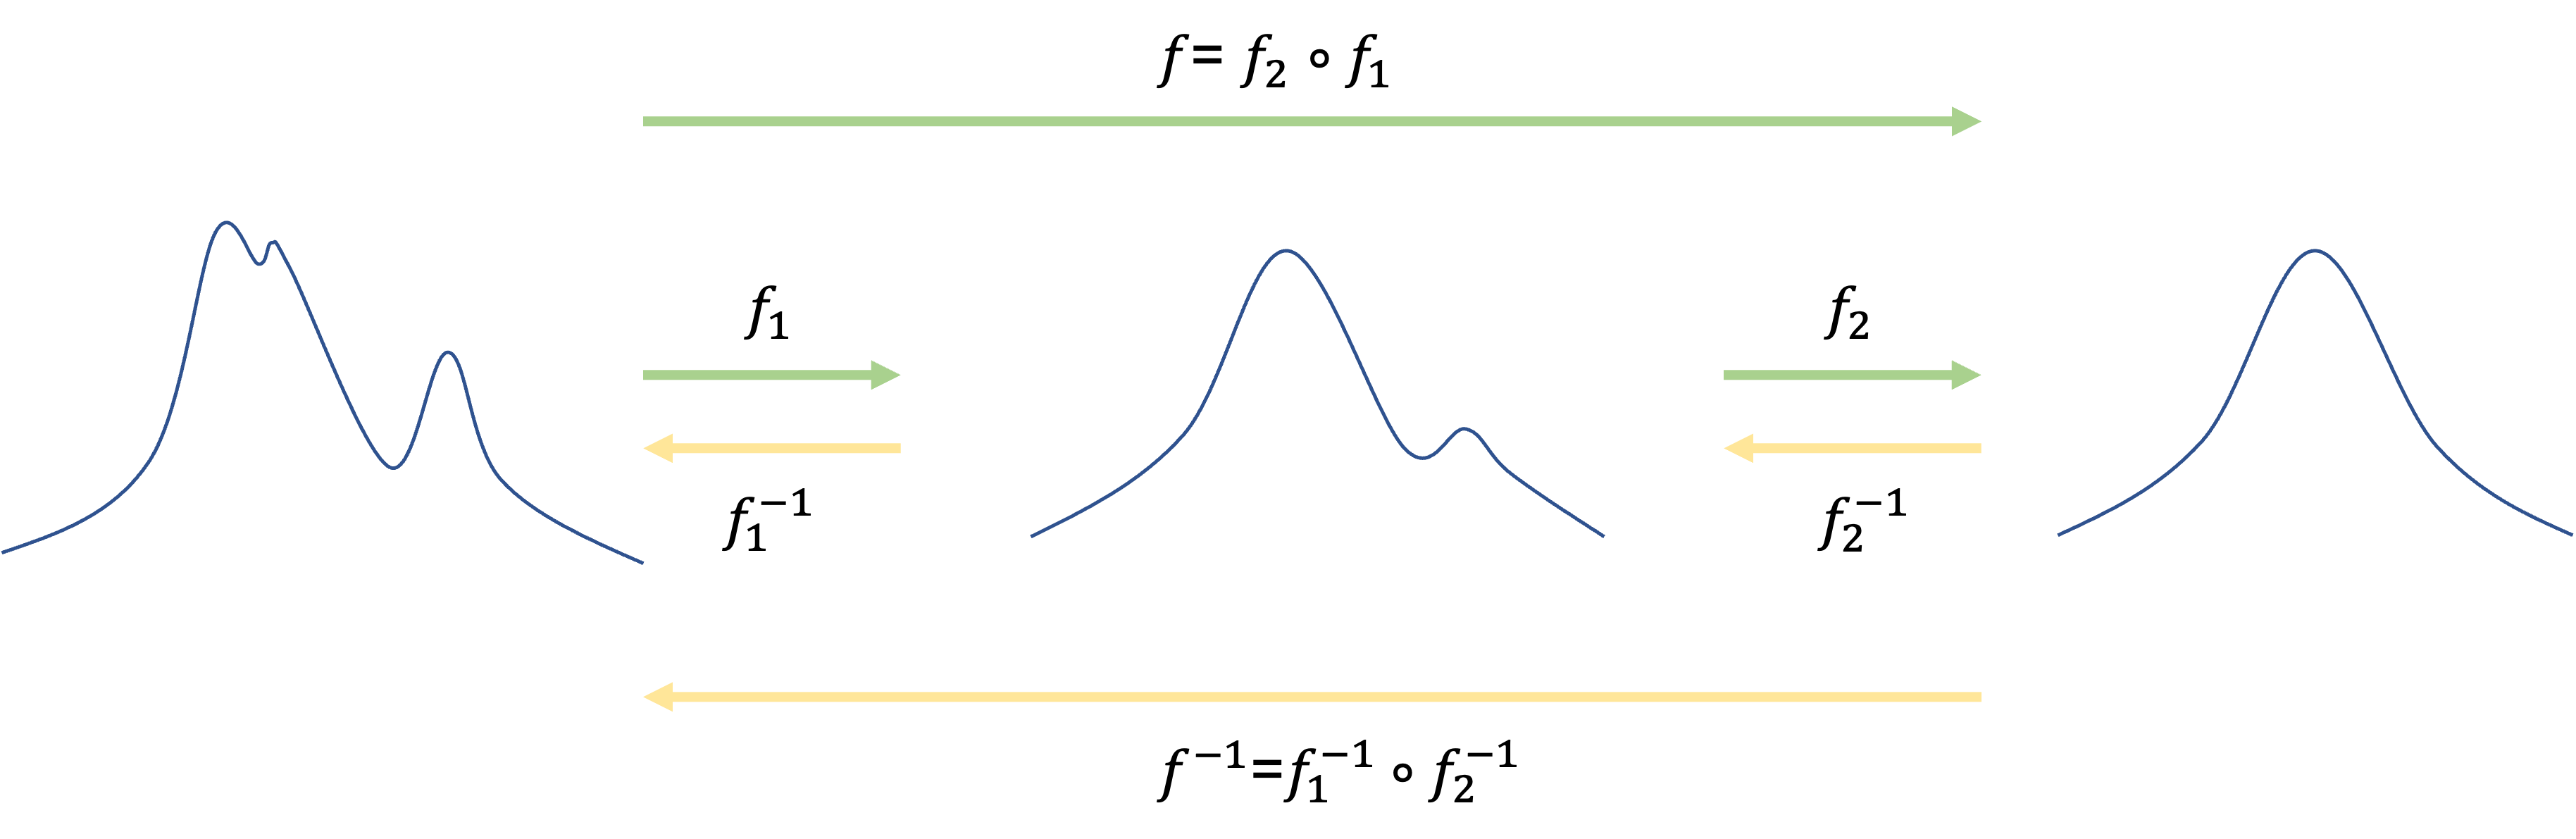
\includegraphics[width=0.8\textwidth]{figures/4/nf-trans.pdf}
    \caption{标准化流原理示意图}
    \label{fig:nf-trans}
\end{figure}

如果变换g能够任意复杂,则可以在对两个分布合理假设下,从任意基分布 $p_{\mathbf{Z}}$生成到任意分布 $p_{\mathbf{Y}}$。该理论经过Bogachev等人证明。\cite{bogachevTriangularTransformationsMeasures2005,medvedevCERTAINPROPERTIESTRIANGULAR2008}


\begin{defn}[双射函数]\label{defn:bio}
	数学中,一个由集合X映射至集合Y的函数,若对每一在Y内的y,存在唯一一个在X内的x与其对应,且对每一在X内的x,存在唯一一个在Y内的y与其对应,则此函数为双射函数。 换句话说,如果其为两集合间的一一对应,则f是双射的。即,同时为单射和满射。
\end{defn}

根据定义\ref{defn:bio},双射函数是可逆函数,但实际情况中构造任意复杂非线性可逆函数(双射)是困难的。人们常说的标准流是指便于计算、求逆和计算雅可比行列式的双射。一种方法是注意可逆函数的组合本身是可逆的,并且其雅可比行列式的行列式具有特定形式。实际上,令 $\mathbf{g}_{1}, \ldots, \mathbf{g}_{N}$是N个双射函数的集合,并且定义 $\mathbf{g}$是这N个双射函数的复合函数,f是它的逆函数,如式\ref{equ:gf}所示。
\begin{quotation}\label{equ:gf}
	\begin{eqnarray}
		\left\{\begin{matrix}
		\mathbf{g} & = & \mathbf{g}_{N} \circ \mathbf{g}_{N-1} \circ \cdots \circ \mathbf{g}_{1}
		\\
		\mathbf{f} & = & \mathbf{f}_{1} \circ \cdots \circ \mathbf{f}_{N-1} \circ \mathbf{f}_{N}
		\end{matrix}\right.
		\end{eqnarray}
\end{quotation}


逆函数f雅可比矩阵的行列式由式\ref{equ:jocob}计算而得。

\begin{equation}\label{equ:jocob}
    \operatorname{det} \operatorname{Df}(\mathbf{y})=\prod_{i=1}^{N} \operatorname{det} \operatorname{D} \mathbf{f}_{i}\left(\mathbf{x}_{i}\right)
\end{equation}

其中 $\operatorname{D}\mathbf{f}_{i}(\mathbf{y})=\frac{\partial \mathbf{f}_{i}}{\partial \mathbf{x}}$是 $\mathbf{f}_{i}$的雅可比矩阵,第i个中间流定义如式\ref{equ:xi},通过复合一系列非线性双射函数来构造出更多复杂函数。
\begin{equation}\label{equ:xi}
	\mathbf{x}_{i}=\mathbf{g}_{i} \circ \cdots \circ \mathbf{g}_{1}(\mathbf{z})=\mathbf{f}_{i+1} \circ \cdots \circ \mathbf{f}_{N}(\mathbf{y}) ,  \mathbf{x}_{N} = \mathbf{y}
\end{equation}

\subsection{概率密度估计和采样} 

标准化流可以用来进行概率密度估计。简单假设只有一个流g,并且g被向量 $\theta$参数化。假设基测度$p_{z}$给定并且被向量$\phi$参数化。给定从复杂分布观测的数据集 $\mathcal{D}=\left\{\mathbf{y}^{(i)}\right\}_{i=1}^{M}$,从而可以基于似然估计参数 $\Theta=(\theta, \phi)$。这个例子中,数据的似然如式\ref{equ:likelihood}所示:
\begin{equation}\label{equ:likelihood}
	\begin{aligned}\log p(\mathcal{D} \mid \Theta) & =\sum_{i=1}^{M} \log p_{\mathbf{Y}}\left(\mathbf{y}^{(i)} \mid \Theta\right) \\& =\sum_{i=1}^{M} \log p_{\mathbf{Z}}\left(\mathbf{f}\left(\mathbf{y}^{(i)} \mid \theta\right) \mid \phi\right)+\log \left|\operatorname{det} \operatorname{Df}\left(\mathbf{y}^{(i)} \mid \theta\right)\right|\end{aligned}
\end{equation}


式\ref{equ:likelihood}中第一行表达式是样本在基测度下的对数似然,第二行表达式,被叫做对数行列式或者体积校正,是用来表示标准化流变换导致的体积变化。在训练中,通过调整流参数 $\theta$和基分布参数$\phi$来最大化对数似然。

评估标准化流建模的分布似然需要计算 f(即标准化方向)和它的对数行列式。在训练中通常需要反复计算似然,因此这些计算的效率尤其重要。然而,从标准化流定义的分布中采样需要评估逆函数g(即生成方向)。因此采样表现表现由生成方向决定。即使流必须是理论上可逆的,逆函数的计算实际上也可能很难。因此,对于概率密度估计,常常是在标准化方向上建模流(即f)。 

\subsection{耦合流}
\begin{figure}[htbp]
    \centering
    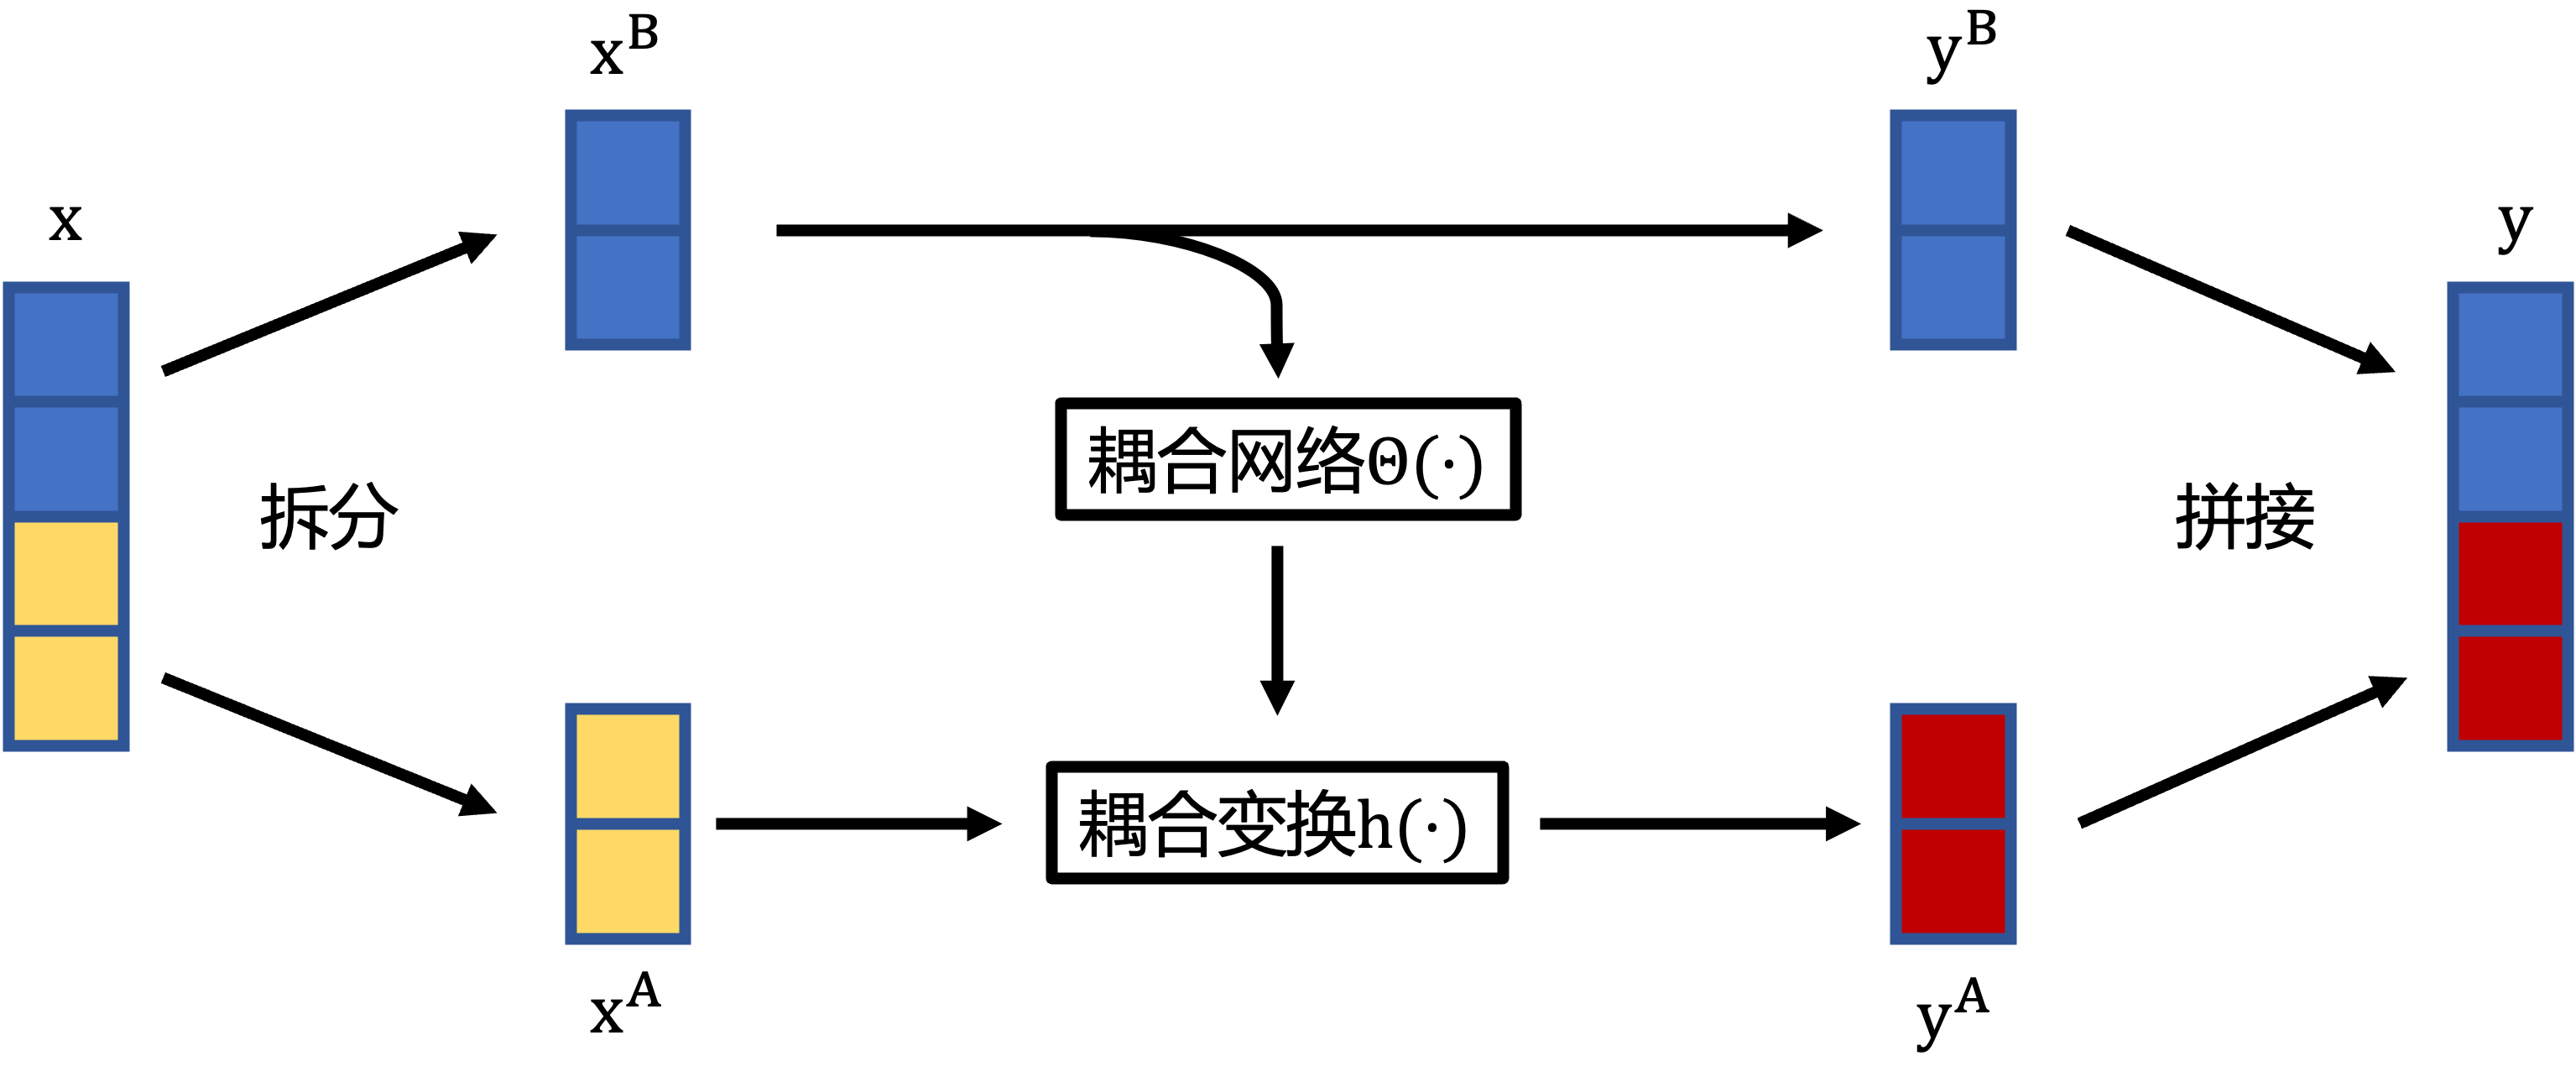
\includegraphics[width=0.75\textwidth]{figures/4/nf-coupling.pdf}
    \caption{耦合流原理示意图}
    \label{fig:nf-coupling}
\end{figure}
为了使标准化流更有计算效率,从而切实可行地来估计概率密度,Dinh等人\cite{dinhNICENonlinearIndependent2015}引入一种耦合的方法为流带来高度表达变换,其原理如图\ref{fig:nf-coupling} 所示。


耦合流将输入 $\mathbf{x} \in \mathbb{R}^{D}$划分为两个子空间 $\left(\mathbf{x}^{A}, \mathbf{x}^{B}\right) \in \mathbb{R}^{d} \times \mathbb{R}^{D-d}$ 并且定义双射函数 $\mathbf{h}(\cdot ; \theta): \mathbb{R}^{d} \rightarrow \mathbb{R}^{d}$,其参数为 $\theta$。定义函数g 如式\ref{equ:coupling-g}所示。
\begin{equation}\label{equ:coupling-g}
    \left\{\begin{matrix}
        \begin{aligned}
        \mathbf{y}^{A} & =\mathbf{h}\left(\mathbf{x}^{A} ; \Theta\left(\mathbf{x}^{B}\right)\right) \\
        \mathbf{y}^{B} & =\mathbf{x}^{B}
        \end{aligned} 
        \end{matrix}\right.
\end{equation}

其中参数 $\theta$定义为只使用 $\mathbf{x}^{B}$作为输入的任一任意函数 $\Theta\left(\mathbf{x}^{B}\right)$。这个函数叫做调节器。双射函数 h 叫做耦合函数,函数g叫做耦合流。一个耦合流是可逆的当且仅当h 是可逆的,其可逆公式如式\ref{equ:converse}所示。

\begin{equation}\label{equ:converse}
    \left\{\begin{matrix}
        \begin{array}{l}\mathbf{x}^{A}=\mathbf{h}^{-1}\left(\mathbf{y}^{A} ; \Theta\left(\mathbf{x}^{B}\right)\right) \\\mathbf{x}^{B}=\mathbf{y}^{B}\end{array}
        \end{matrix}\right.
\end{equation}

g的雅可比矩阵是分块三角矩阵,对角块分别是 $\operatorname{D}\mathbf{h}$和单位阵。因此耦合层雅可比矩阵的行列式就简化为 $\operatorname{D}\mathbf{h}$的行列式,如式\ref{equ:h}所示。

\begin{equation}\label{equ:h}
    \mathbf{h}\left(\mathbf{x}^{A} ; \theta\right)=\left(h_{1}\left(x_{1}^{A} ; \theta_{1}\right), \ldots, h_{d}\left(x_{d}^{A} ; \theta_{d}\right)\right)
\end{equation}


大多数耦合函数是按元素应用到$\mathbf{x}^{A}$,如式。其中每个 $h_{i}\left(\cdot ; \theta_{i}\right): \mathbb{R} \rightarrow \mathbb{R}$是一个标量双射。在这种情况下一个耦合流是一个三角变换(即有一个三角雅可比矩阵)。

耦合流的调节器$\Theta\left(\mathbf{x}^{B}\right)$可以是任意复杂,这是其关键变量。在实际应用中,通常将调节器建模为一个神经网络。

此外,调节器可以是不变的(即完全不依赖 $\mathbf{x}^{B}$),从而实现构建多尺度流。Dinh等人\cite{lelanPerfectDensityModels2021}在生成方向的分布引入了维度。在标准化方向,这个维度每个迭代步骤减半,这样大部分语义信息保留。这减少了转换高维分布的计算成本并且可以捕获某些类型的数据 (例如自然图像) 中固有的多尺度结构。

如何划分x是耦合流的另一个变量,通常在将输入随机排列后进行对半划分。除此之外还有一些常见的结构划分操作,例如,在非体积保持流中的图像的情况下,使用交替像素或通道块的“掩膜”流。

\subsection{仿射耦合函数} 

NICE\cite{dinhNICENonlinearIndependent2015}、RealNVP\cite{dinhDensityEstimationUsing2017}、Glow\cite{kingmaGlowGenerativeFlow2018}使用仿射耦合函数来实现耦合流,其简单、易于计算而且能表示复杂的分布。仿射耦合函数 $h: \mathbb{R} \rightarrow \mathbb{R}$的定义如式\ref{equ:hxtheta}所示。
\begin{equation}\label{equ:hxtheta}
    h(x ; \theta)=\theta_{1} x+\theta_{2}, \quad \theta_{1} \neq 0, \theta_{2} \in \mathbb{R} .
\end{equation}


L2范数利用网络的中间层的特征图提取的特征向量符合多元高斯分布的先验假设。本文采用上述耦合函数构成的标准化流进行概率密度估计,标准化流的输入 $x \in \mathbb{R}^{w \times h \times n_{\text {feat }}}$是尺寸为 $w \times h$有 $n_{feat}$特征的特征图。在这些块中。在随机选择保持固定的排列之后,输入 $x$的通道沿着通道均匀地划分为部分 $\mathbf{x}^{A}$和 $\mathbf{x}^{B}$。这些部分中的每一个作为静态条件都与位置编码c拼接。

为了充分利用所有信息,一般对两部分交替进行仿射变换。本文通过为每个部分建立 $s_{i}$和 $t_{i}$的子网络来实现仿射变换,如式\ref{equ:y2y1}所示。

\begin{equation}\label{equ:y2y1}
    \left\{\begin{matrix}
        \begin{array}{c}y_{2}=x_{2} \odot e^{s_{1}\left(\left[x_{1}, c\right]\right)}+t_{1}\left(\left[x_{1}, c\right]\right) \\y_{1}=x_{1} \odot e^{s_{2}\left(\left[x_{2}, c\right]\right)}+t_{2}\left(\left[x_{2}, c\right]\right)\end{array}
        \end{matrix}\right.
\end{equation}

其中 $\odot$是元素的乘积, $\left[ ·,·\right]$表示沿通道拼接。一个耦合块的输出是沿着通道对$y_{1}$和$y_{2}$的拼接,输入和输出的维数保持一致。

\subsection{位置编码} 

在仿射耦合函数应用标准化流的基础上,本文还参考CFLOW-AD\cite{gudovskiyCFLOWADRealTimeUnsupervised2022}的做法引入条件变量,用位置编码 $\boldsymbol{c}_{pos} \in \mathbb{R}^{D}, pos \in\left\{w \times h\right\}$拼接解码器耦合层的中间变量从而扩展了无条件流框架。

位置编码的实现方法参考Transformer\cite{vaswaniAttentionAllYou2017}中提出的方法,使用如式\ref{equ:positionencoder}所示的不同频率正弦和余弦函数。

\begin{equation}\label{equ:positionencoder}
    \left\{\begin{matrix}
    \begin{aligned}P E_{(p o s, 2 d)} & =\sin \left(\frac{p o s}{10000^{\frac{2 d}{n_{\text {feat }}}}}  \right) \\P E_{(p o s, 2 d+1)} & =\cos \left(\frac{p o s}{10000^{\frac{2 d}{n_{\text {feat }}}}}  \right)\end{aligned}
\end{matrix}\right.
\end{equation}

其中 pos是位置,d是维度。每个位置编码的维度都对应一个正弦。考虑对每一个固定的偏移k, $P E_{p o s+k}$能够表示为 $P E_{p o s}$的线性函数,CFLOW-AD假设该函数对模型按相对位置学习是有益的。

此外,在Transformer中实验的表明,使用通过学习获得的位置嵌入和通过正弦获得嵌入的效果相差不大,但选择正弦版本可以在推广模型到对其它长度序列进行位置编码时减少训练量。


\begin{figure}[htbp]
    \centering
    \includegraphics[width=0.9\textwidth]{figures/4/teacher.pdf}
    \caption{教师网络结构}
    \label{fig:nf-teacher}
\end{figure}

教师网络结构如图\ref{fig:nf-teacher}所示。使用变量公式的变化z作为最终输出如式\ref{equ:px}所示。

\begin{equation}\label{equ:px}
    p_{X}(x)=p_{Z}(z)\left|\operatorname{det} \frac{\partial z}{\partial x}\right|
\end{equation}

生成模型的目标就是对目标数据的分布进行建模,其通常利用极大似然估计或最小化某些差异来评估。教师网络以 $p_{Z}$为正态分布 $\mathcal{N}(0, I)$ ,通过优化在像素位置 $(i,j)$全部前景像素的均值来最小化负对数似然,教师网络损失如式\ref{equ:teacherloss}所示。本文不直接以教师网络输出计算异常分数,而是将训练教师网络作为训练学生网络的前置任务。

\begin{equation}\label{equ:teacherloss}
    \mathcal{L}_{i j}^{t}=-\log p_{X}\left(x_{i j}\right)=\frac{\left\|z_{i j}\right\|_{2}^{2}}{2}-\log \left|\operatorname{det} \frac{\partial z_{i j}}{\partial x_{i j}}\right|
\end{equation}


\section{学生网络}
本文采用异构的教师学生网络组合,学生网络是一个包含残差块的简单全卷积网络,而没有采用教师网络的可逆变换。学生网络的每个残差块由3×3卷积层的两个序列组成,利用批归一化\cite{ioffeBatchNormalizationAccelerating2015}和leaky ReLU激活。学生网络在残差块前后各设一层卷积来保证特征维度与教师网络一致。

在网络输入阶段,本文将深度图像和其HOG特征在输入学生网络前先拼接,然后再经过两层专门为深度特征混合图的卷积层来提取深度图的特征,最后再和RGB特征一起通过卷积层融合然后输入残差块。学生网络结构如图\ref{fig:student}所示
\begin{figure}[htbp]
    \centering
    \includegraphics[width=0.9\textwidth]{figures/4/student.pdf}
    \caption{学生网络结构}
    \label{fig:student}
\end{figure}

此外,位置编码c在输入学生网络前进行了拼接,其输出维度与教师匹配从而实现逐像素的距离计算。学生网络的目标是最小化在训练样本 $x \in X$的学生输出 $f_{s}(x)$和教师输出 $f_{t}(x)$之间的  $\ell_{2} \text {-distance }$的平方。给定训练集 $X$,在像素位置 $(i,j)$的输出如式\ref{equ:studentloss}所示。

\begin{equation}\label{equ:studentloss}
    \mathcal{L}_{i j}^{s}=\left\|f_{s}(x)_{i j}-f_{t}(x)_{i j}\right\|_{2}^{2}   
\end{equation}


在所有(前景)像素上平均 $\mathcal{L}_{i j}^{s}$即可得到最后的损失 $\mathcal{L}^{s}$,其也被用于计算排除背景像素的图像级异常得分,本文通过计算像素上的最大值或平均值来聚合一个样本的像素距离。
\section{实验设计及结果分析}
\subsection{数据集}
本文使用第二章搭建的实验平台,对实验室的塑料工件进行拍摄,采集用于训练和验证的数据。首先是采集正常样本,实验平台按照设定从多个角度全自动采集出192组图像,每组图像均由RGB图像和深度图像组成,其中部分正常样本组如图\ref{fig:normal-smaple}所示。
\begin{figure}[htbp]
    \centering
    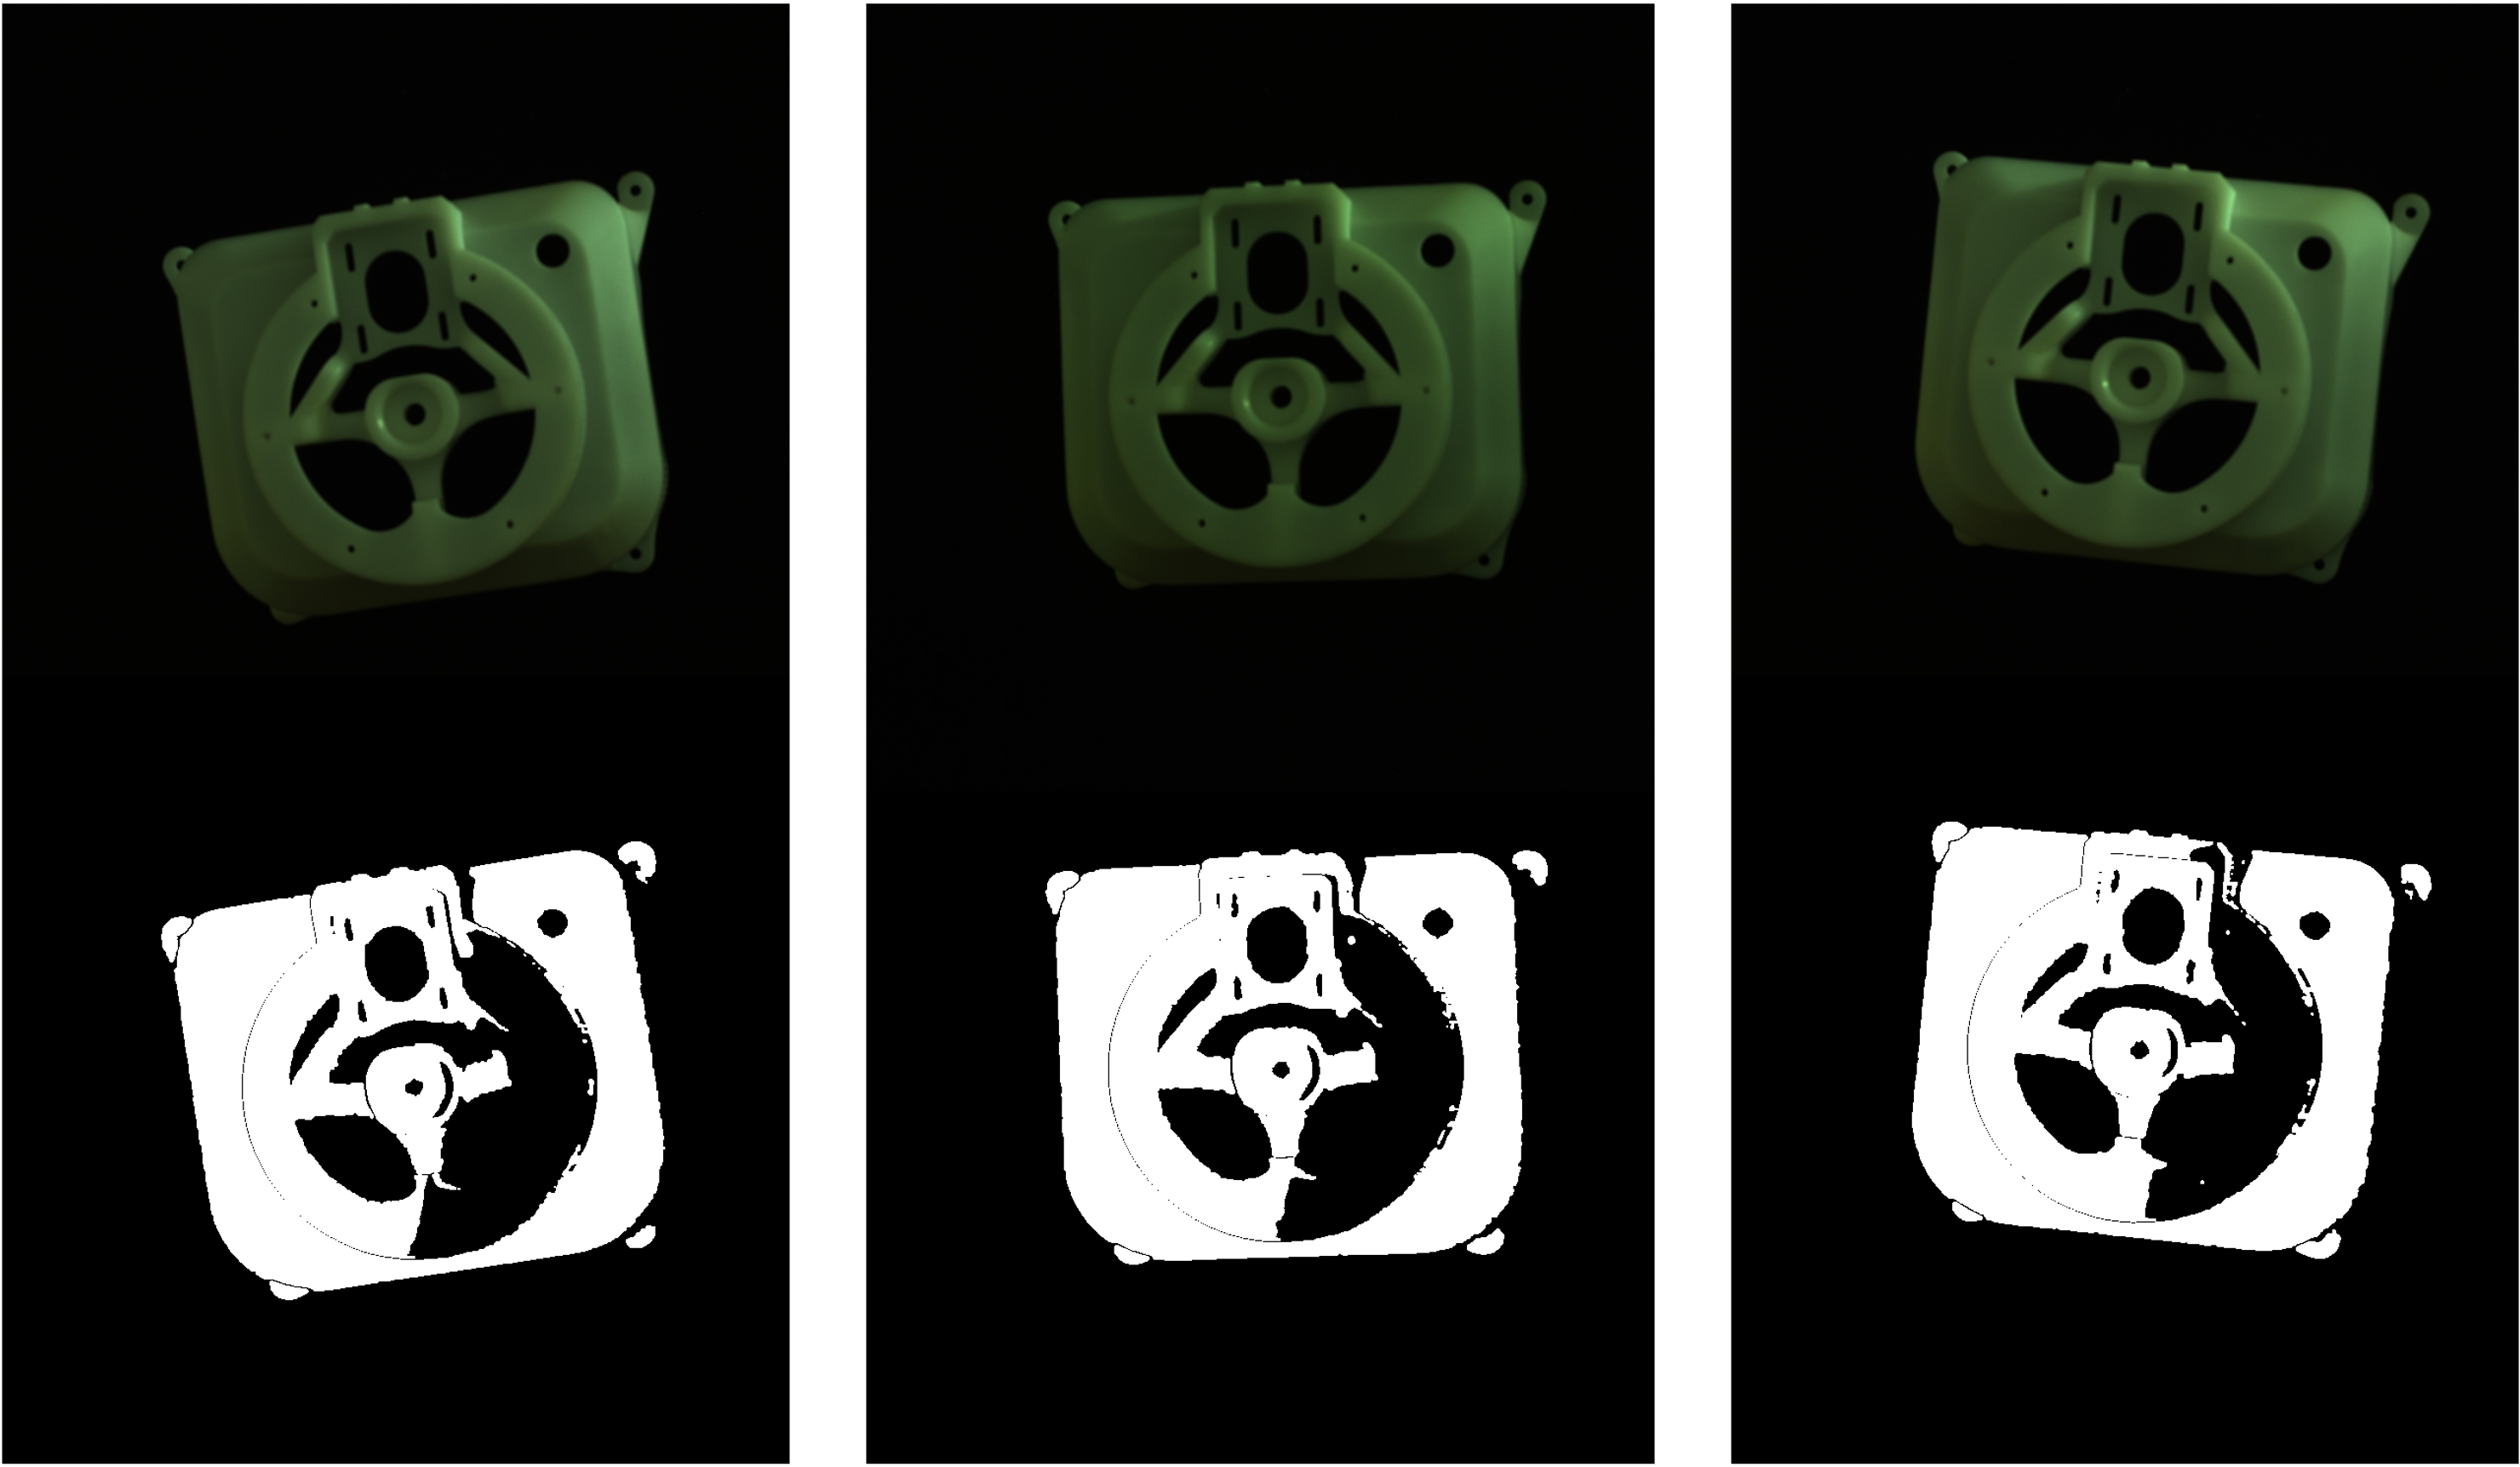
\includegraphics[width=0.75\textwidth]{figures/4/normal-smaple.png}
    \caption{正常样本}
    \label{fig:normal-smaple}
\end{figure}

为了检验本文的多模态缺陷算法的性能,本文又通过手工制造了三类五种缺陷模拟可能存在的缺陷类型,这些缺陷样本总共有96组。其中第一类缺陷为结构变型缺陷,包括横向和纵向变型,如图\ref{fig:bad-1}所示,其中左图为横向变型,右图为纵向变型。
\begin{figure}[htbp]
    \centering
    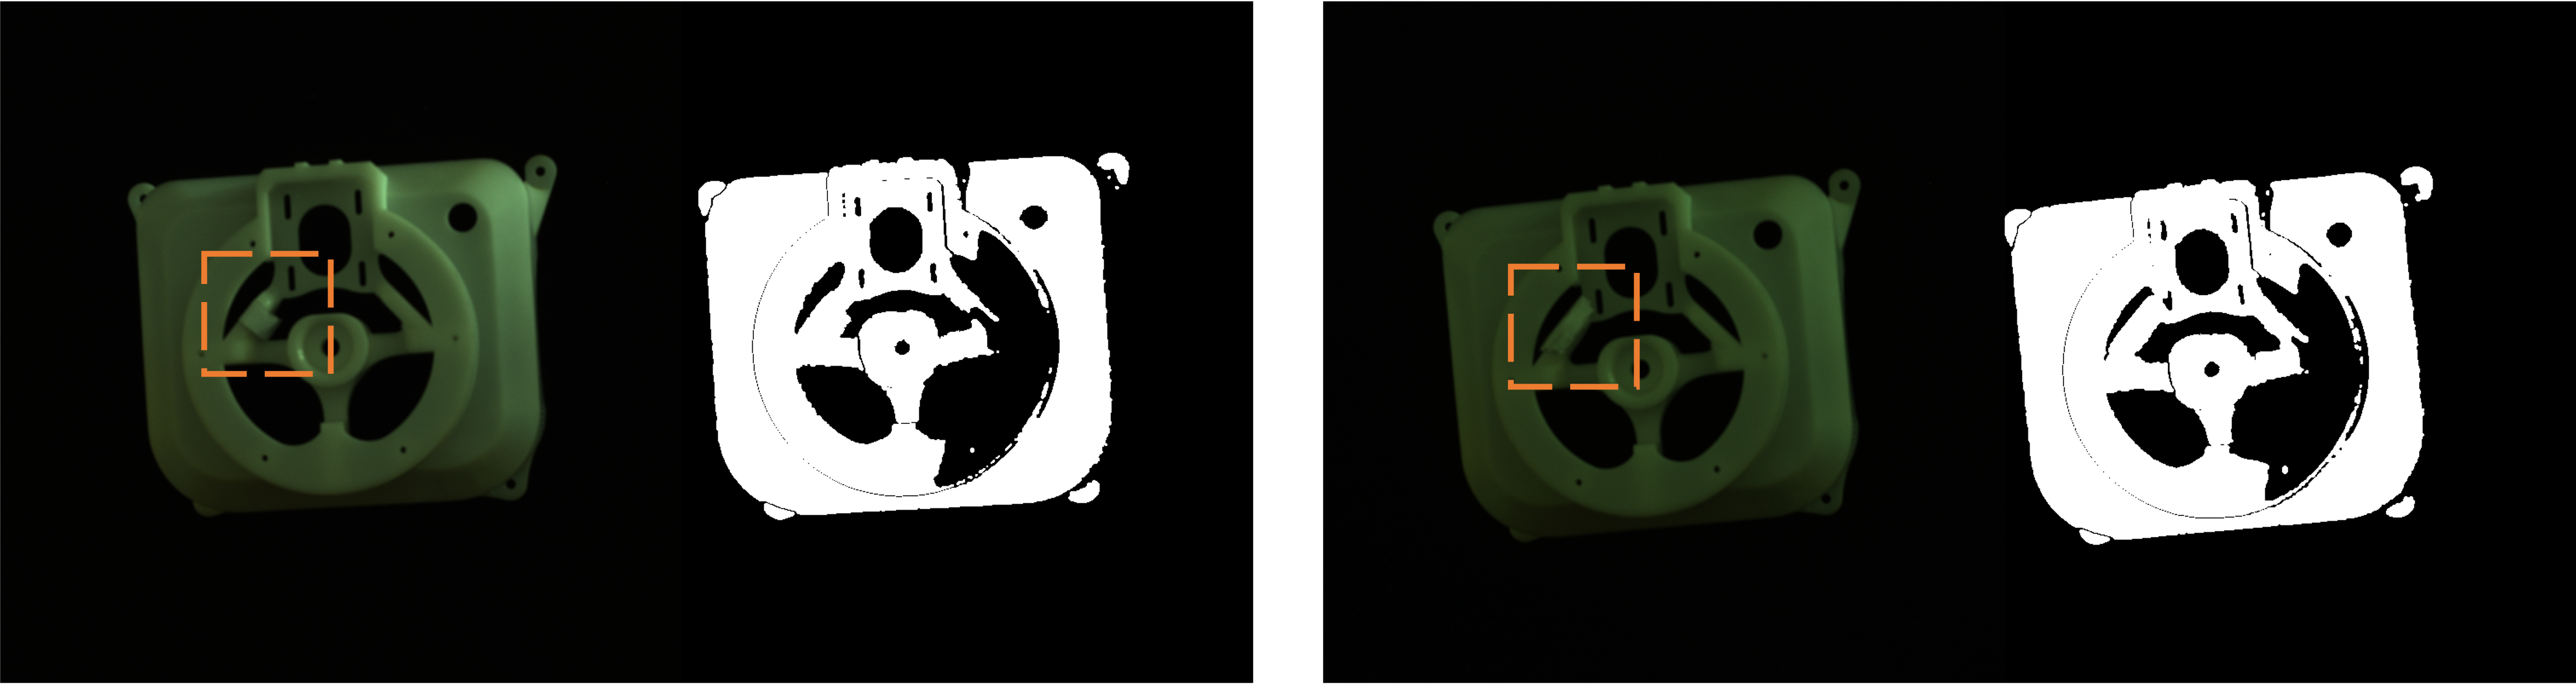
\includegraphics[width=1\textwidth]{figures/4/bad-1.png}
    \caption{结构变型缺陷}
    \label{fig:bad-1}
\end{figure}

第二类缺陷为空洞填充缺陷,如图\ref{fig:bad-2}所示,其中左图展示的整个空洞完全填充的缺陷,右图展示的是空洞单侧填充的缺陷。
\begin{figure}[htbp]
    \centering
    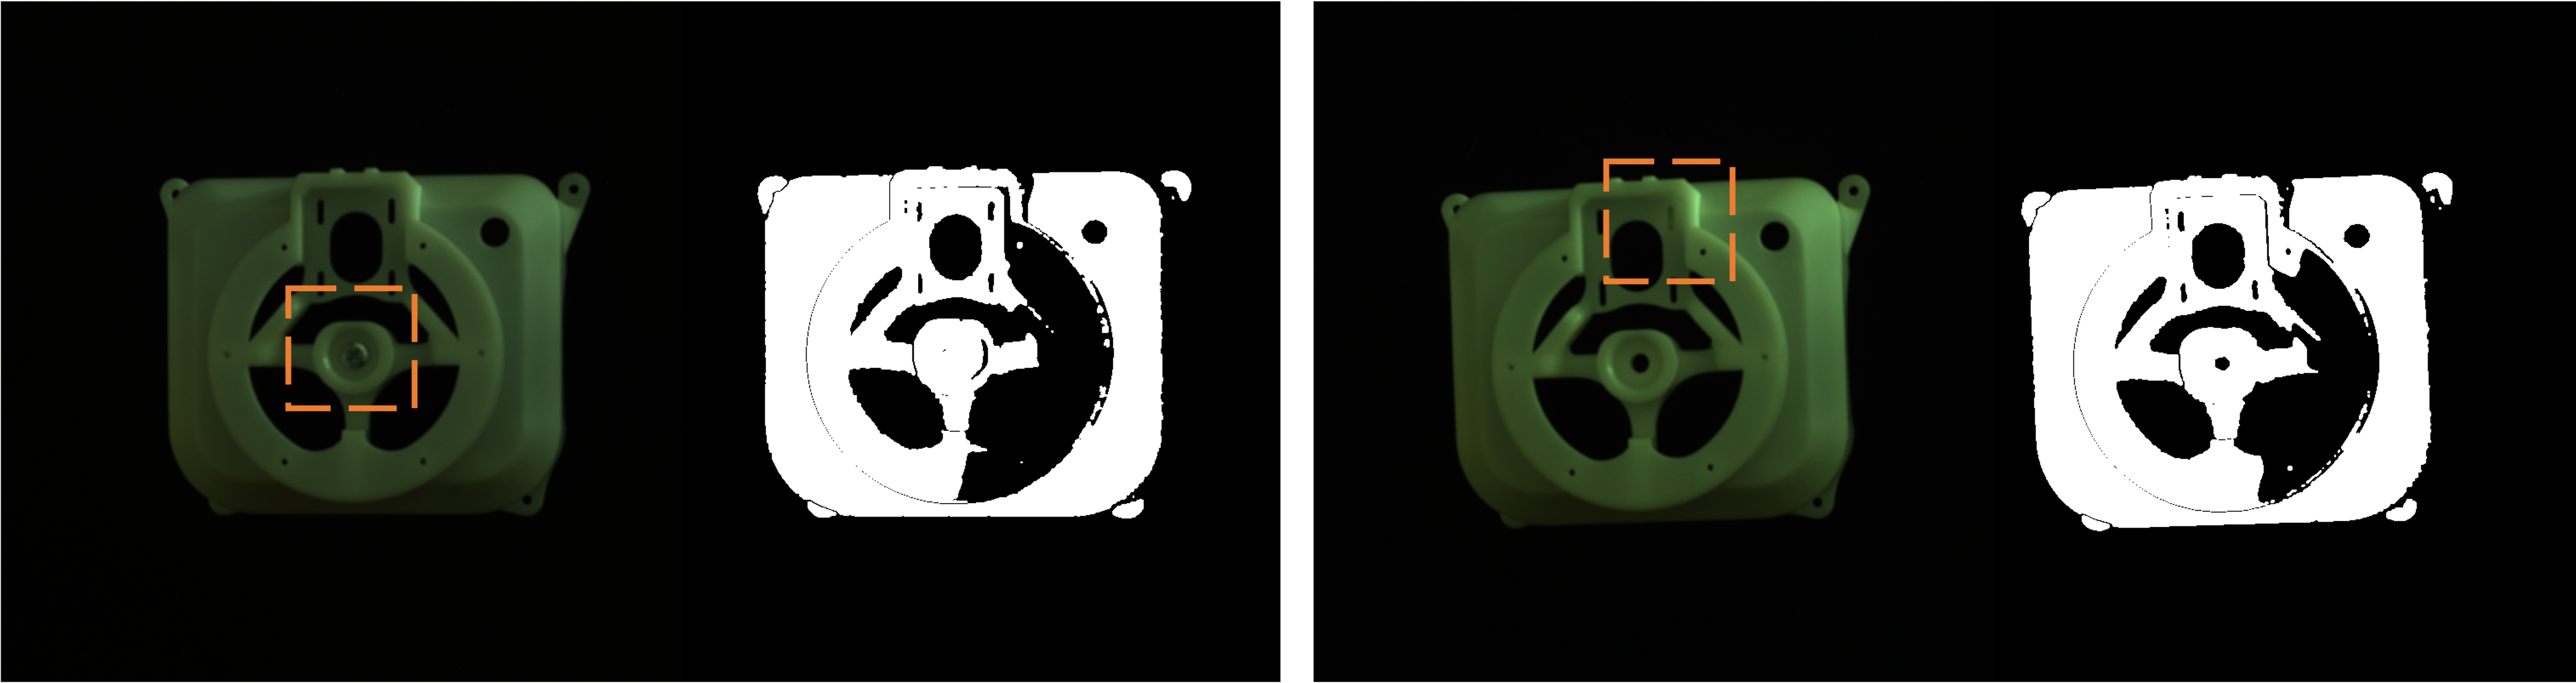
\includegraphics[width=1\textwidth]{figures/4/bad-2.png}
    \caption{空洞填充缺陷}
    \label{fig:bad-2}
\end{figure}

第三类缺陷为划痕和杂色缺陷,如图\ref{fig:bad-3}中的红色浅划痕。
\begin{figure}[htbp]
    \centering
    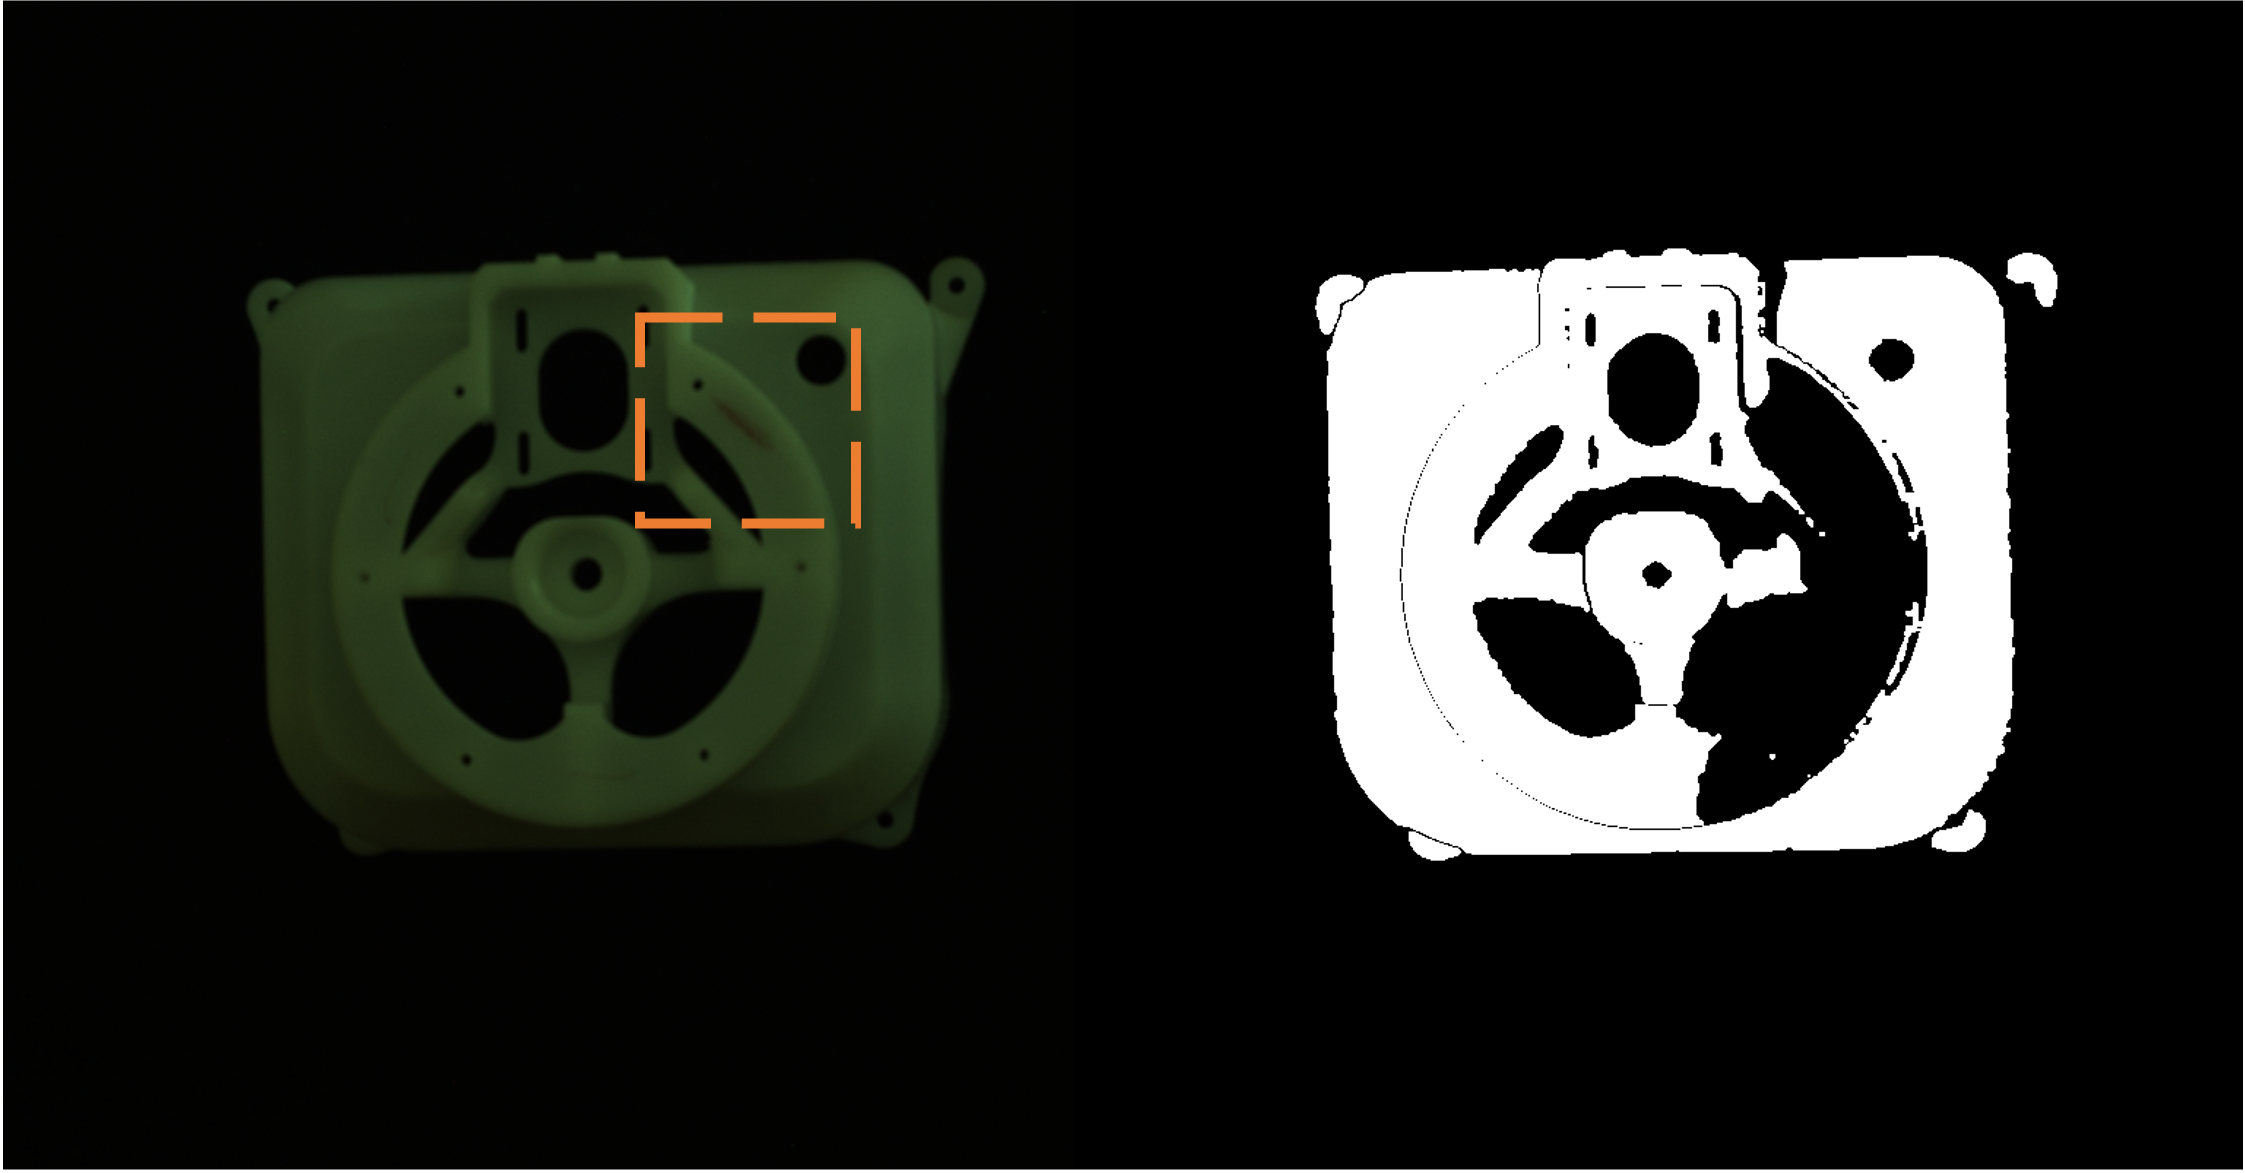
\includegraphics[width=0.6\textwidth]{figures/4/bad-3.png}
    \caption{划痕和杂色缺陷}
    \label{fig:bad-3}
\end{figure}

本文将上述正常样本和缺陷样本组合建立用于模型训练和验证的数据集,数据集的结构表\ref{tab:4-dataset}所示。
\begin{table}[htbp]
    \centering
    \caption{数据集} \label{tab:4-dataset}
    \begin{tabular*}{0.75\textwidth}{@{\extracolsep{\fill}}ccc}
    \toprule
    %   数据集&正常样本&变型缺陷&填充缺陷&划痕杂色缺陷&混合缺陷\\
    % \midrule
    %   训练集&160&-&-	&-&- \\
    %   测试集	&32	&32 &32	&16&16			 \\
      &正常样本&缺陷样本\\
      \midrule
        训练集&160&-\\
        测试集	&32&96\\
      
    \bottomrule
    \end{tabular*}
\end{table}
\subsection{实验设计}
根据对输入深度图像值处理的方式不同,本文设计了四个对比实验,如表\ref{tab:4-experiment-desgin}所示。其中AST是原始模型,通过对深度图像原始像素进行块混合下采样的方式来使深度图像与预训练的RGB特征图维数匹配;H-AST是在AST的基础上引入HOG对深度图像进行特征提取后再在维度上进行拼接;F-AST是对输入学生网络的深度图像先进行两层卷积后再与RGB特征图拼接然后输入残差块;HF-AST则是结合HOG和学生网络卷积层对深度图像特征提取。其中HF-AST是本文提出的新方法,H-AST和F-AST是对该方法的一个消融实验。
\begin{table}[htbp]
    \centering
    \caption{实验设计} \label{tab:4-experiment-desgin}
    \begin{tabular*}{0.6\textwidth}{@{\extracolsep{\fill}}cc}
    \toprule
      缺陷检测算法&深度图处理方式\\
      \midrule
        AST&像素值混合\\
        H-AST	&HOG\\
        F-AST&学生网络卷积\\
        HF-AST	&HOG+学生网络卷积\\
      
    \bottomrule
    \end{tabular*}
\end{table}

\subsection{实验结果分析}
\begin{figure}[htbp]
    \centering
    \begin{subfigure}
        \centering
        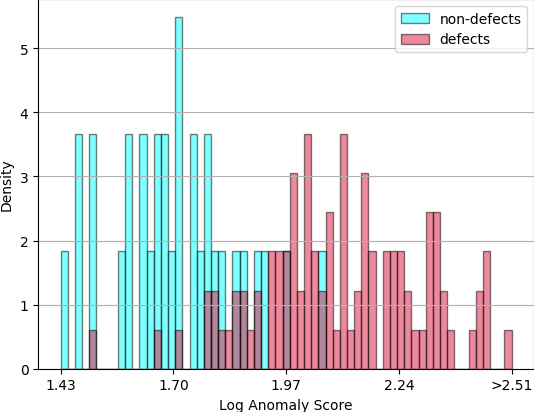
\includegraphics[width=.4\linewidth]{figures/4/hist/ori_experiment/plastics_mean.png}  
      \end{subfigure}
      \begin{subfigure}
        \centering
        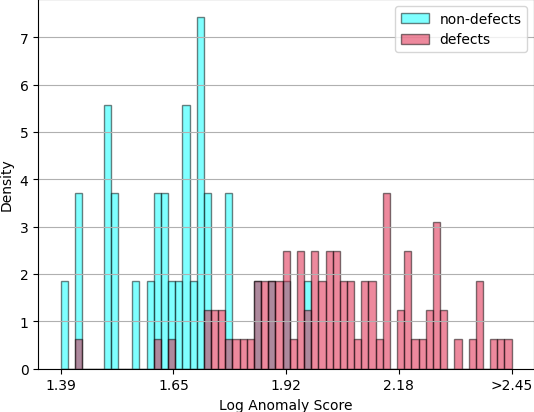
\includegraphics[width=.4\linewidth]{figures/4/hist/hog_experiment/plastics_mean.png} 
      \end{subfigure}
      \begin{subfigure}
        \centering
        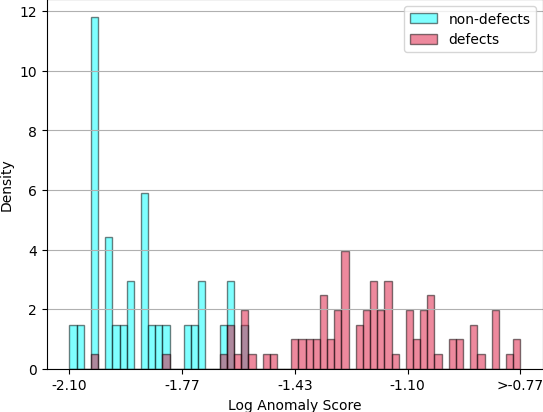
\includegraphics[width=.4\linewidth]{figures/4/hist/mix_experiment/plastics_mean.png} 
      \end{subfigure}
      \begin{subfigure}
        \centering
        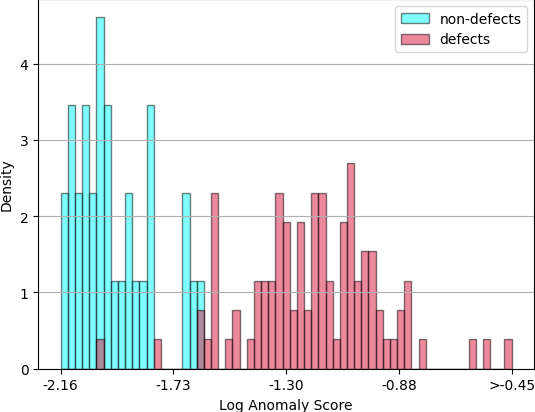
\includegraphics[width=.4\linewidth]{figures/4/hist/mixhog_experiment/plastics_mean.png} 
      \end{subfigure}
    \caption{平均直方图}
    \label{fig:hist_mean}
\end{figure}
按照实验设计,本文进行多次实验,每次实验所有方法除对深度图像处理方法有所差异外,其余各项参数均保持一致。针对本文的多模态缺陷检测,本文分别采用了平均距离和最大距离来计算图像级异常得分,实验结果如下列图像所示。其中直方图用于统计测试集异常得分情况,蓝色柱表示测试集中正常样本的异常得分分布,红色柱则表示缺陷样本。AUROC图则是衡量缺陷检测算法性能的指标。在每组图片中,左上为AST,右上为H-AST,左下为F-AST,右下为HF-AST。

组图\ref{fig:hist_mean}是根据平均距离计算测试集对数异常得分的统计直方图。从组图中可以看到表示正常样本的蓝色柱和表示缺陷样本的红色柱呈现两个不同分布,但同时两者有所相交。

\begin{figure}[htbp]
    \centering
    \begin{subfigure}
        \centering
        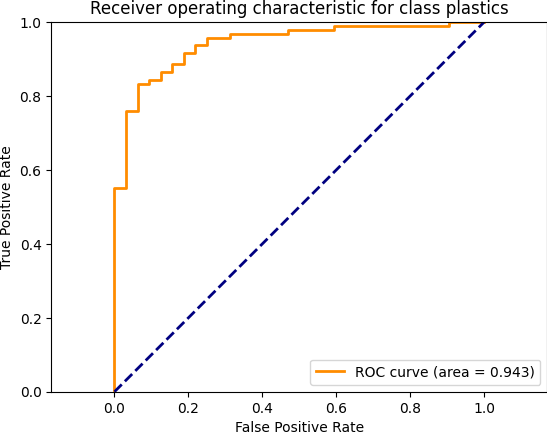
\includegraphics[width=.4\linewidth]{figures/4/auroc/ori_experiment/plastics_mean.png}  
        \end{subfigure}
        \begin{subfigure}
        \centering
        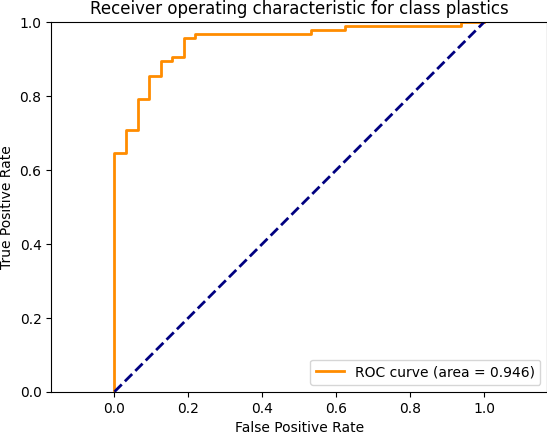
\includegraphics[width=.4\linewidth]{figures/4/auroc/hog_experiment/plastics_mean.png} 
        \end{subfigure}
        \begin{subfigure}
        \centering
        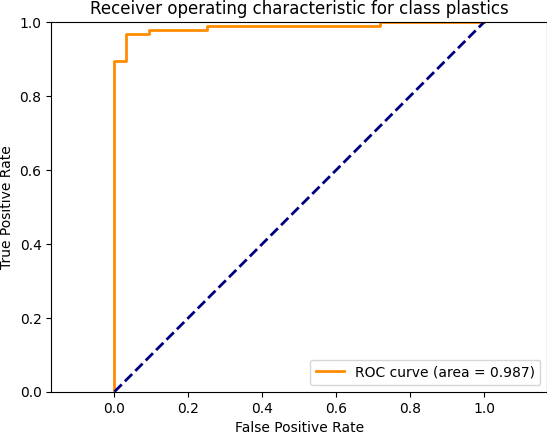
\includegraphics[width=.4\linewidth]{figures/4/auroc/mix_experiment/plastics_mean.png} 
        \end{subfigure}
        \begin{subfigure}
        \centering
        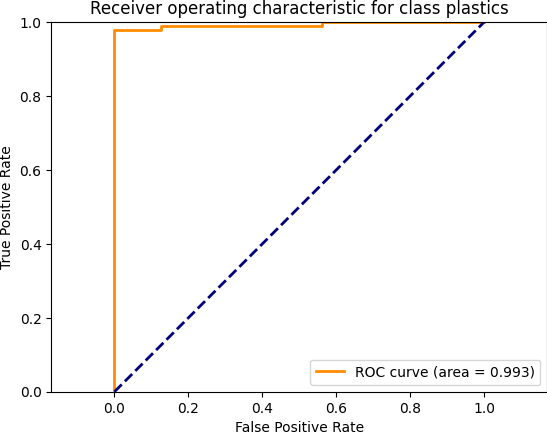
\includegraphics[width=.4\linewidth]{figures/4/auroc/mixhog_experiment/plastics_mean.png} 
        \end{subfigure}
    \caption{平均AUROC}
    \label{fig:auroc_mean}
    \end{figure}
组图\ref{fig:auroc_mean}是根据平均距离计算的AUROC。从图中可以看出本文实验的所有方法采用平均距离衡量均能取得不错的表现,HF-AST方法在平均距离计算异常得分下实现99.3\%的AUROC,超过其它方法。此外,H-AST和AST以及HF-AST和F-AST的两组实验对比说明加入HOG能够对算法有小幅提升;F-AST和AST以及HF-AST和H-AST的两组实验对比说明使用在学生网络加入深度图像卷积层对缺陷检测性能提升明显。


\begin{figure}[htbp]
\centering
\begin{subfigure}
    \centering
    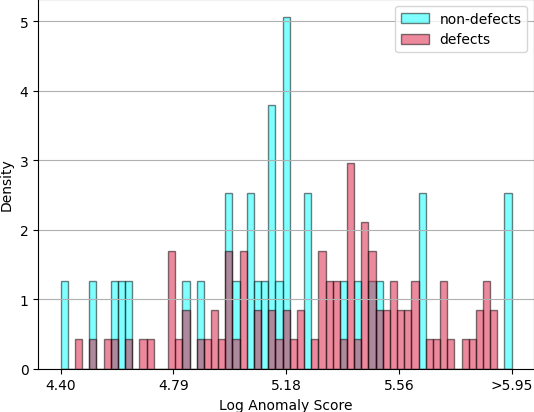
\includegraphics[width=.4\linewidth]{figures/4/hist/ori_experiment/plastics_max.png}  
    \end{subfigure}
    \begin{subfigure}
    \centering
    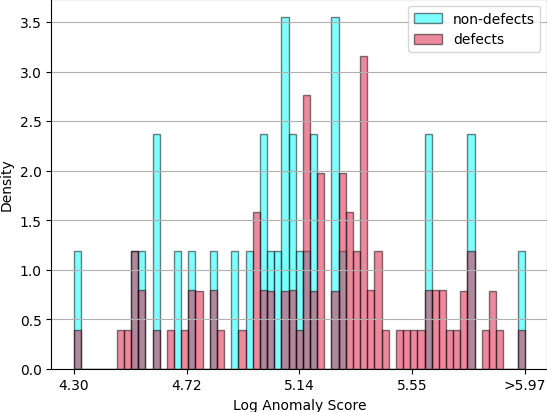
\includegraphics[width=.4\linewidth]{figures/4/hist/hog_experiment/plastics_max.png} 
    \end{subfigure}
    \begin{subfigure}
    \centering
    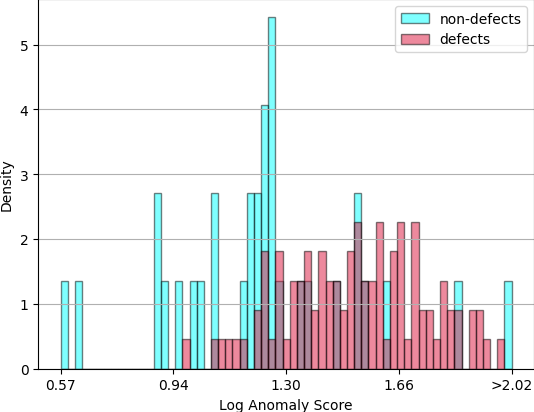
\includegraphics[width=.4\linewidth]{figures/4/hist/mix_experiment/plastics_max.png} 
    \end{subfigure}
    \begin{subfigure}
    \centering
    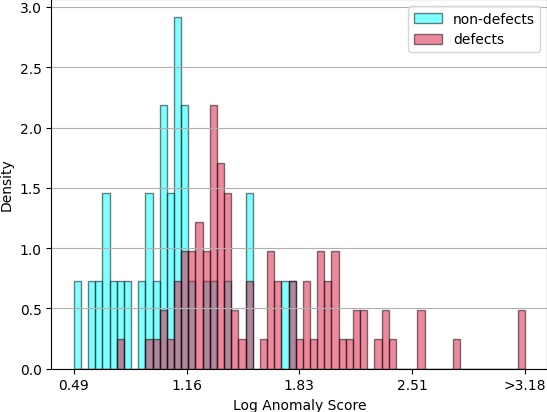
\includegraphics[width=.4\linewidth]{figures/4/hist/mixhog_experiment/plastics_max.png} 
    \end{subfigure}
\caption{最大直方图}
\label{fig:hist_max}
\end{figure}

\begin{figure}[htbp]
    \centering
    \begin{subfigure}
        \centering
        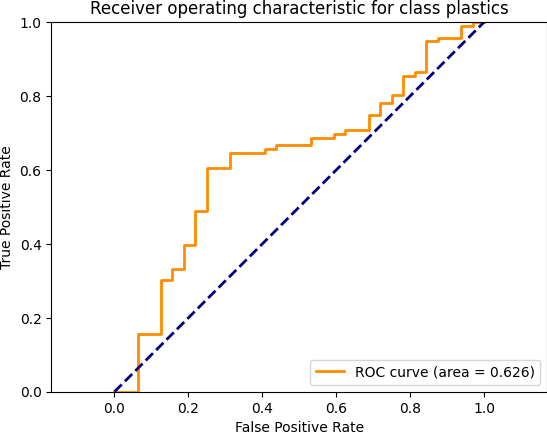
\includegraphics[width=.4\linewidth]{figures/4/auroc/ori_experiment/plastics_max.png}  
        \end{subfigure}
        \begin{subfigure}
        \centering
        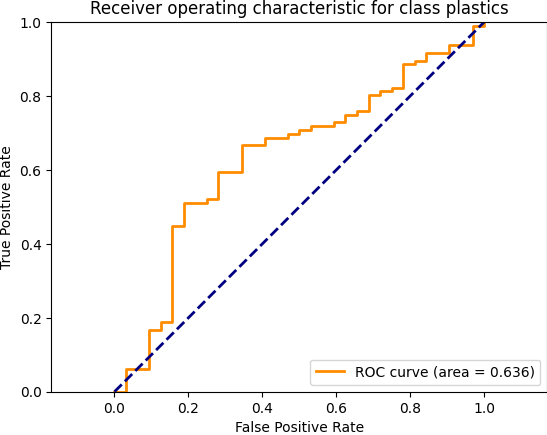
\includegraphics[width=.4\linewidth]{figures/4/auroc/hog_experiment/plastics_max.png} 
        \end{subfigure}
        \begin{subfigure}
        \centering
        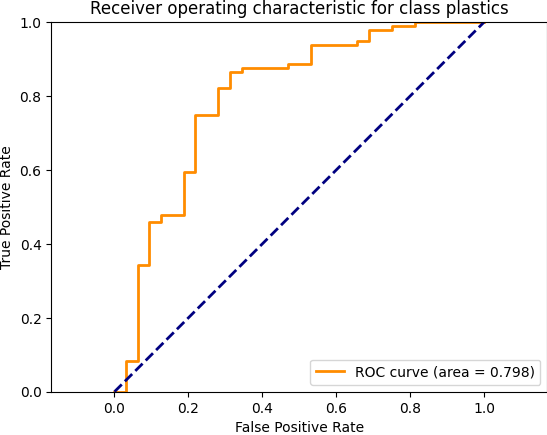
\includegraphics[width=.4\linewidth]{figures/4/auroc/mix_experiment/plastics_max.png} 
        \end{subfigure}
        \begin{subfigure}
        \centering
        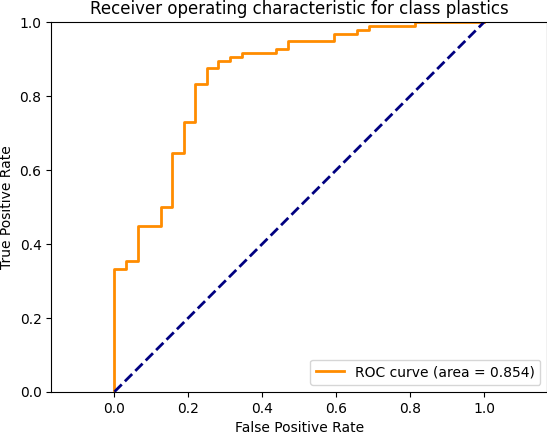
\includegraphics[width=.4\linewidth]{figures/4/auroc/mixhog_experiment/plastics_max.png} 
        \end{subfigure}
    \caption{最大AUROC}
    \label{fig:auroc_max}
    \end{figure}
组图\ref{fig:hist_max}是根据最大距离计算测试集对数异常得分的统计直方图。从组图中可以看到未引入学生网络深度图像卷积层的原模型的正常样本和缺陷样本分布相近,影响是否有缺陷分类的准确性。


组图\ref{fig:auroc_max}是根据最大距离计算的AUROC。从图中可以看出本文实验的所有方法相较于用平均距离衡量的性能方差要大,HF-AST方法在最大距离计算异常得分下实现85.4\%的AUROC,远超过其它方法。此外,H-AST和AST以及HF-AST和F-AST的两组实验对比说明在引入学生网络深度图像卷积下,加入HOG能够对算法性能提升更为有效;F-AST和AST以及HF-AST和H-AST的两组实验对比说明使用在学生网络加入深度图像卷积层对缺陷检测性能提升显著。

汇总上述实验结果为表\ref{tab:plastics-experiment} ,该表展现了本文提出的改进异构教师学生网络在本文的塑料件上性能提升明显。
\begin{table}[htbp]
    \centering
    \caption{塑料件数据集实验结果} \label{tab:plastics-experiment}
    \begin{tabular*}{0.8\textwidth}{@{\extracolsep{\fill}}ccccc}
    \toprule
      &AST&H-AST&F-AST&HF-AST\\
      \midrule
      mean AUROC&0.943&0.946&0.987&0.993\\
      max AUROC&0.626&0.636&0.798&0.854\\
    \bottomrule
    \end{tabular*}
\end{table}

最后,本文分别应用原始AST模型和本文提出改进的HF-AST模型对空洞填充和结构变型缺陷样本进行缺陷检测并生成热力图。其中组图\ref{fig:featmap-1}是空洞填充缺陷,组图\ref{fig:featmap-2}是结构变型缺陷。组图的第一行分别是输入的RGB图像和深度图像,虚线框包围的是热力图,热力图中颜色越黄则表示该处异常得分越高。

\begin{figure}[htbp]
    \centering
    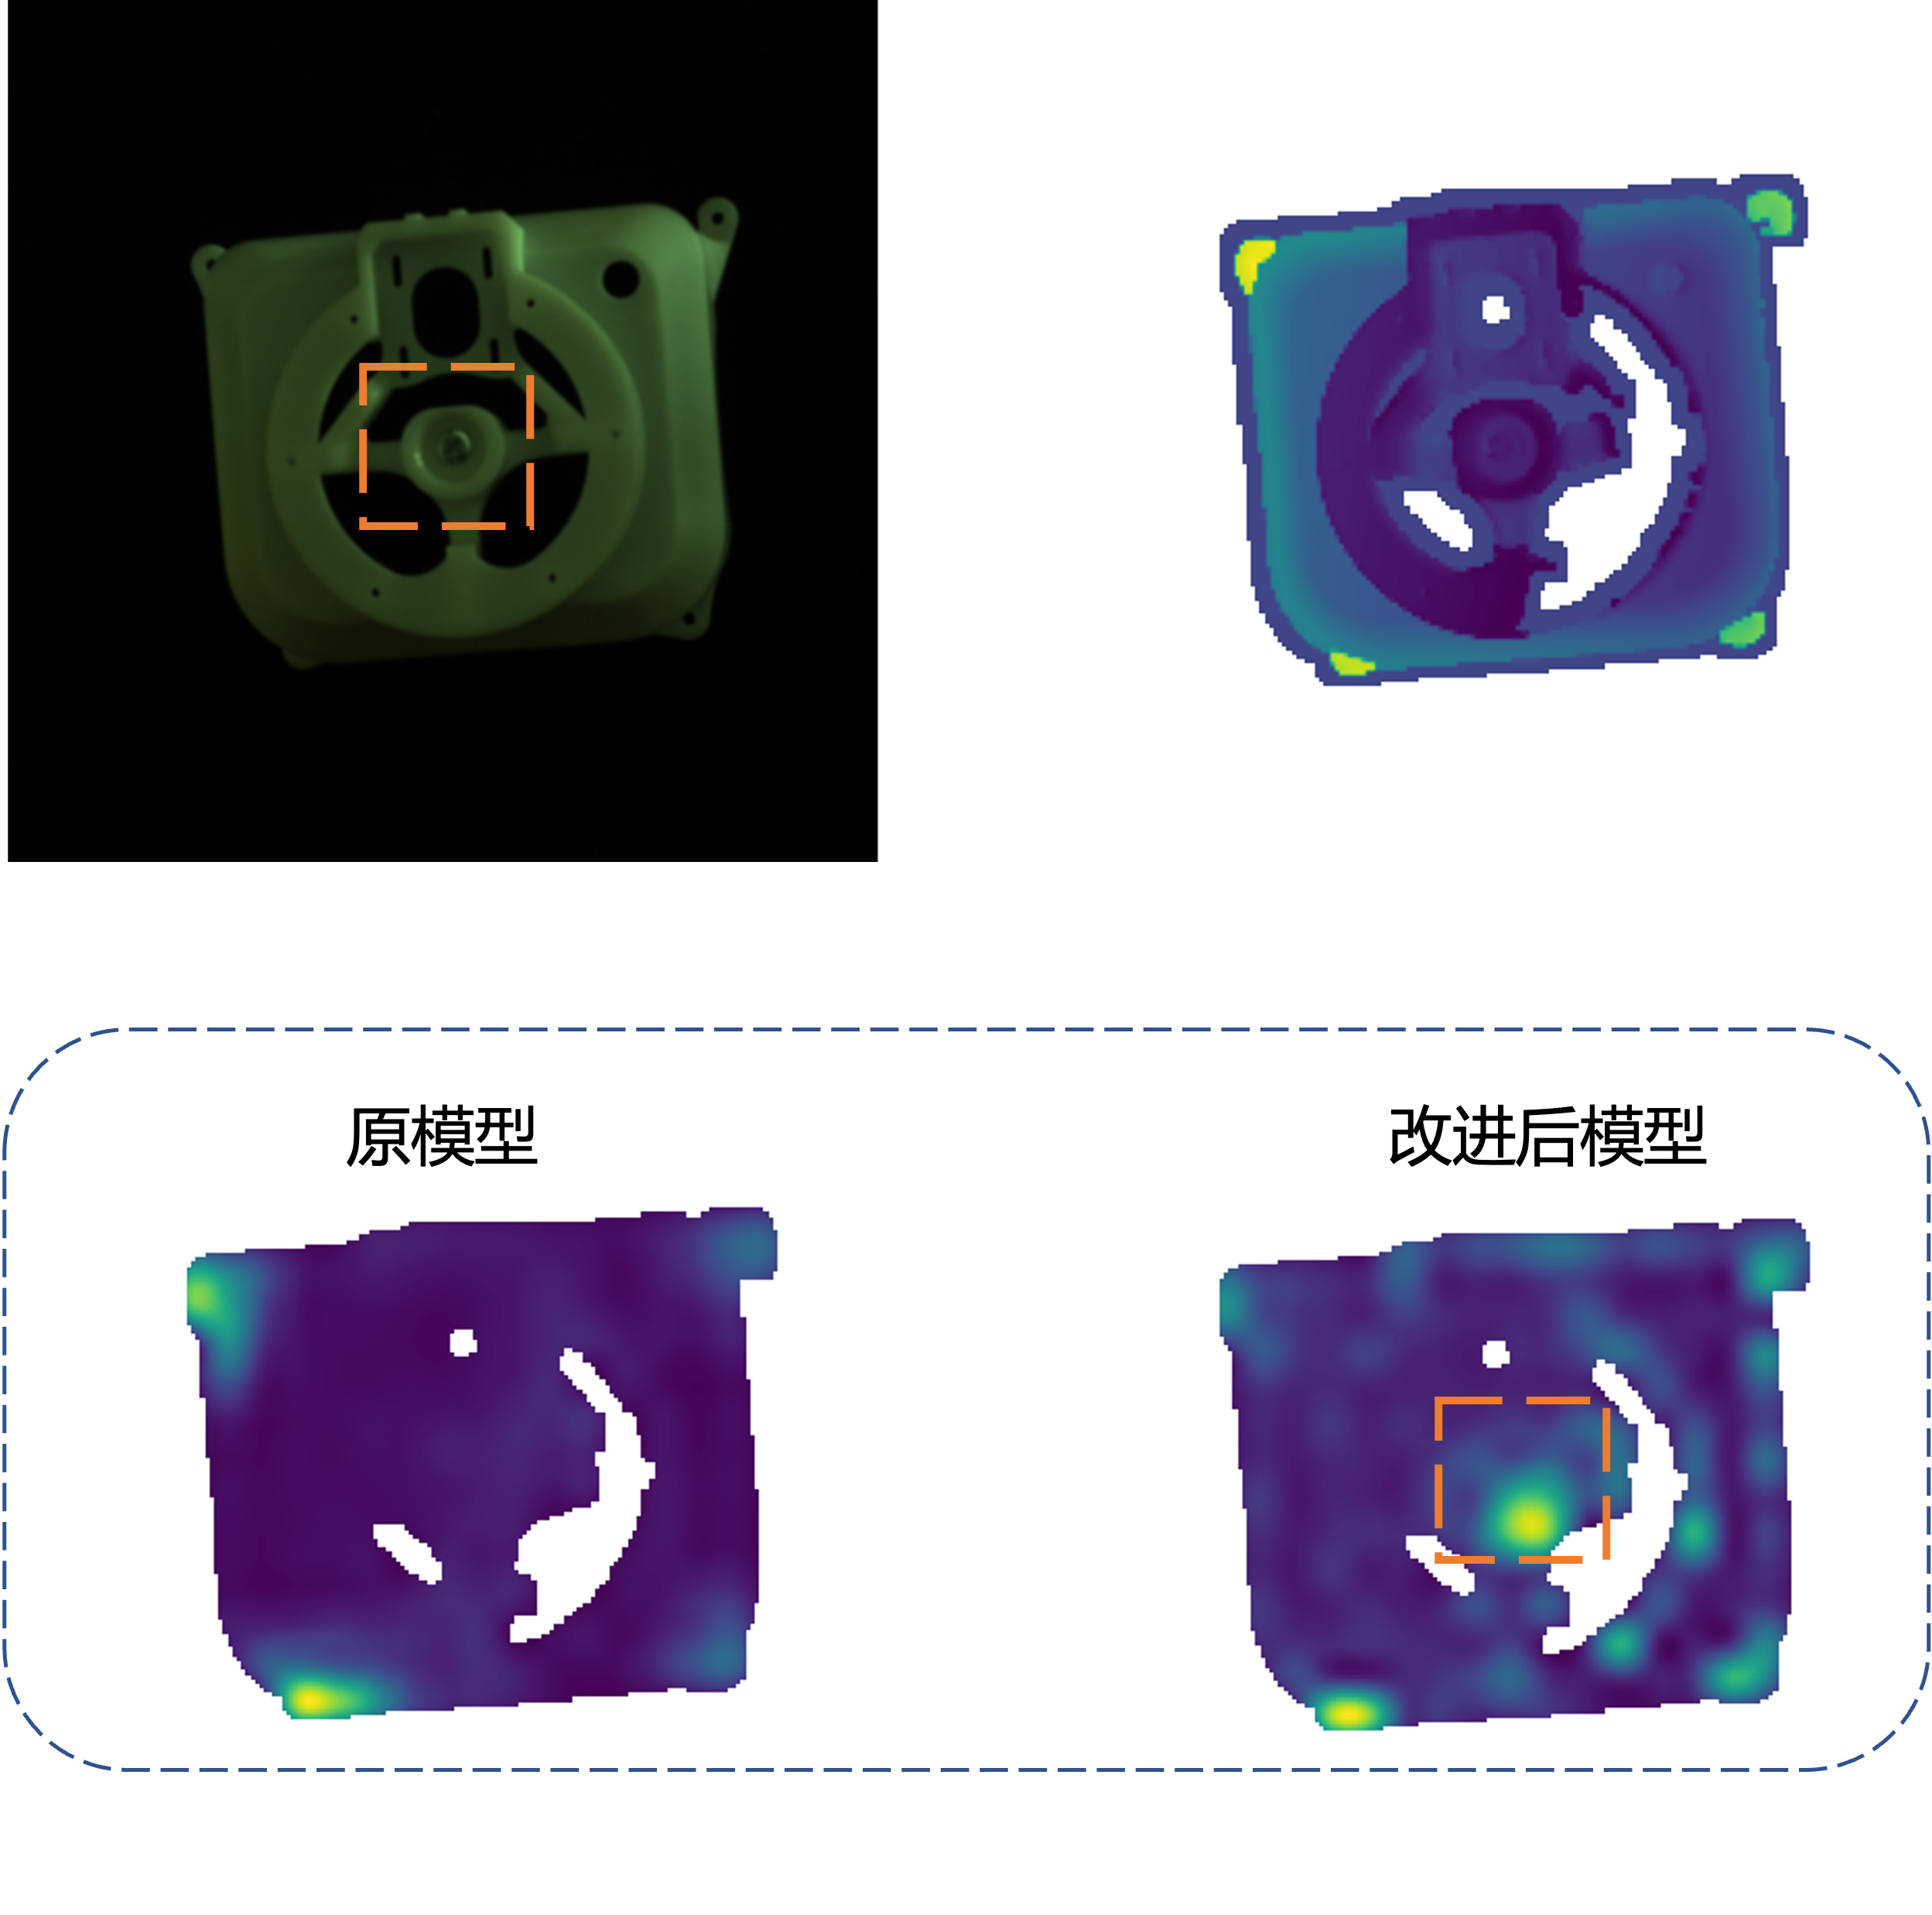
\includegraphics[width=0.6\textwidth]{figures/4/featmap-1.png}
    \caption{空洞填充热力图}
    \label{fig:featmap-1}
\end{figure}

\begin{figure}[htbp]
    \centering
    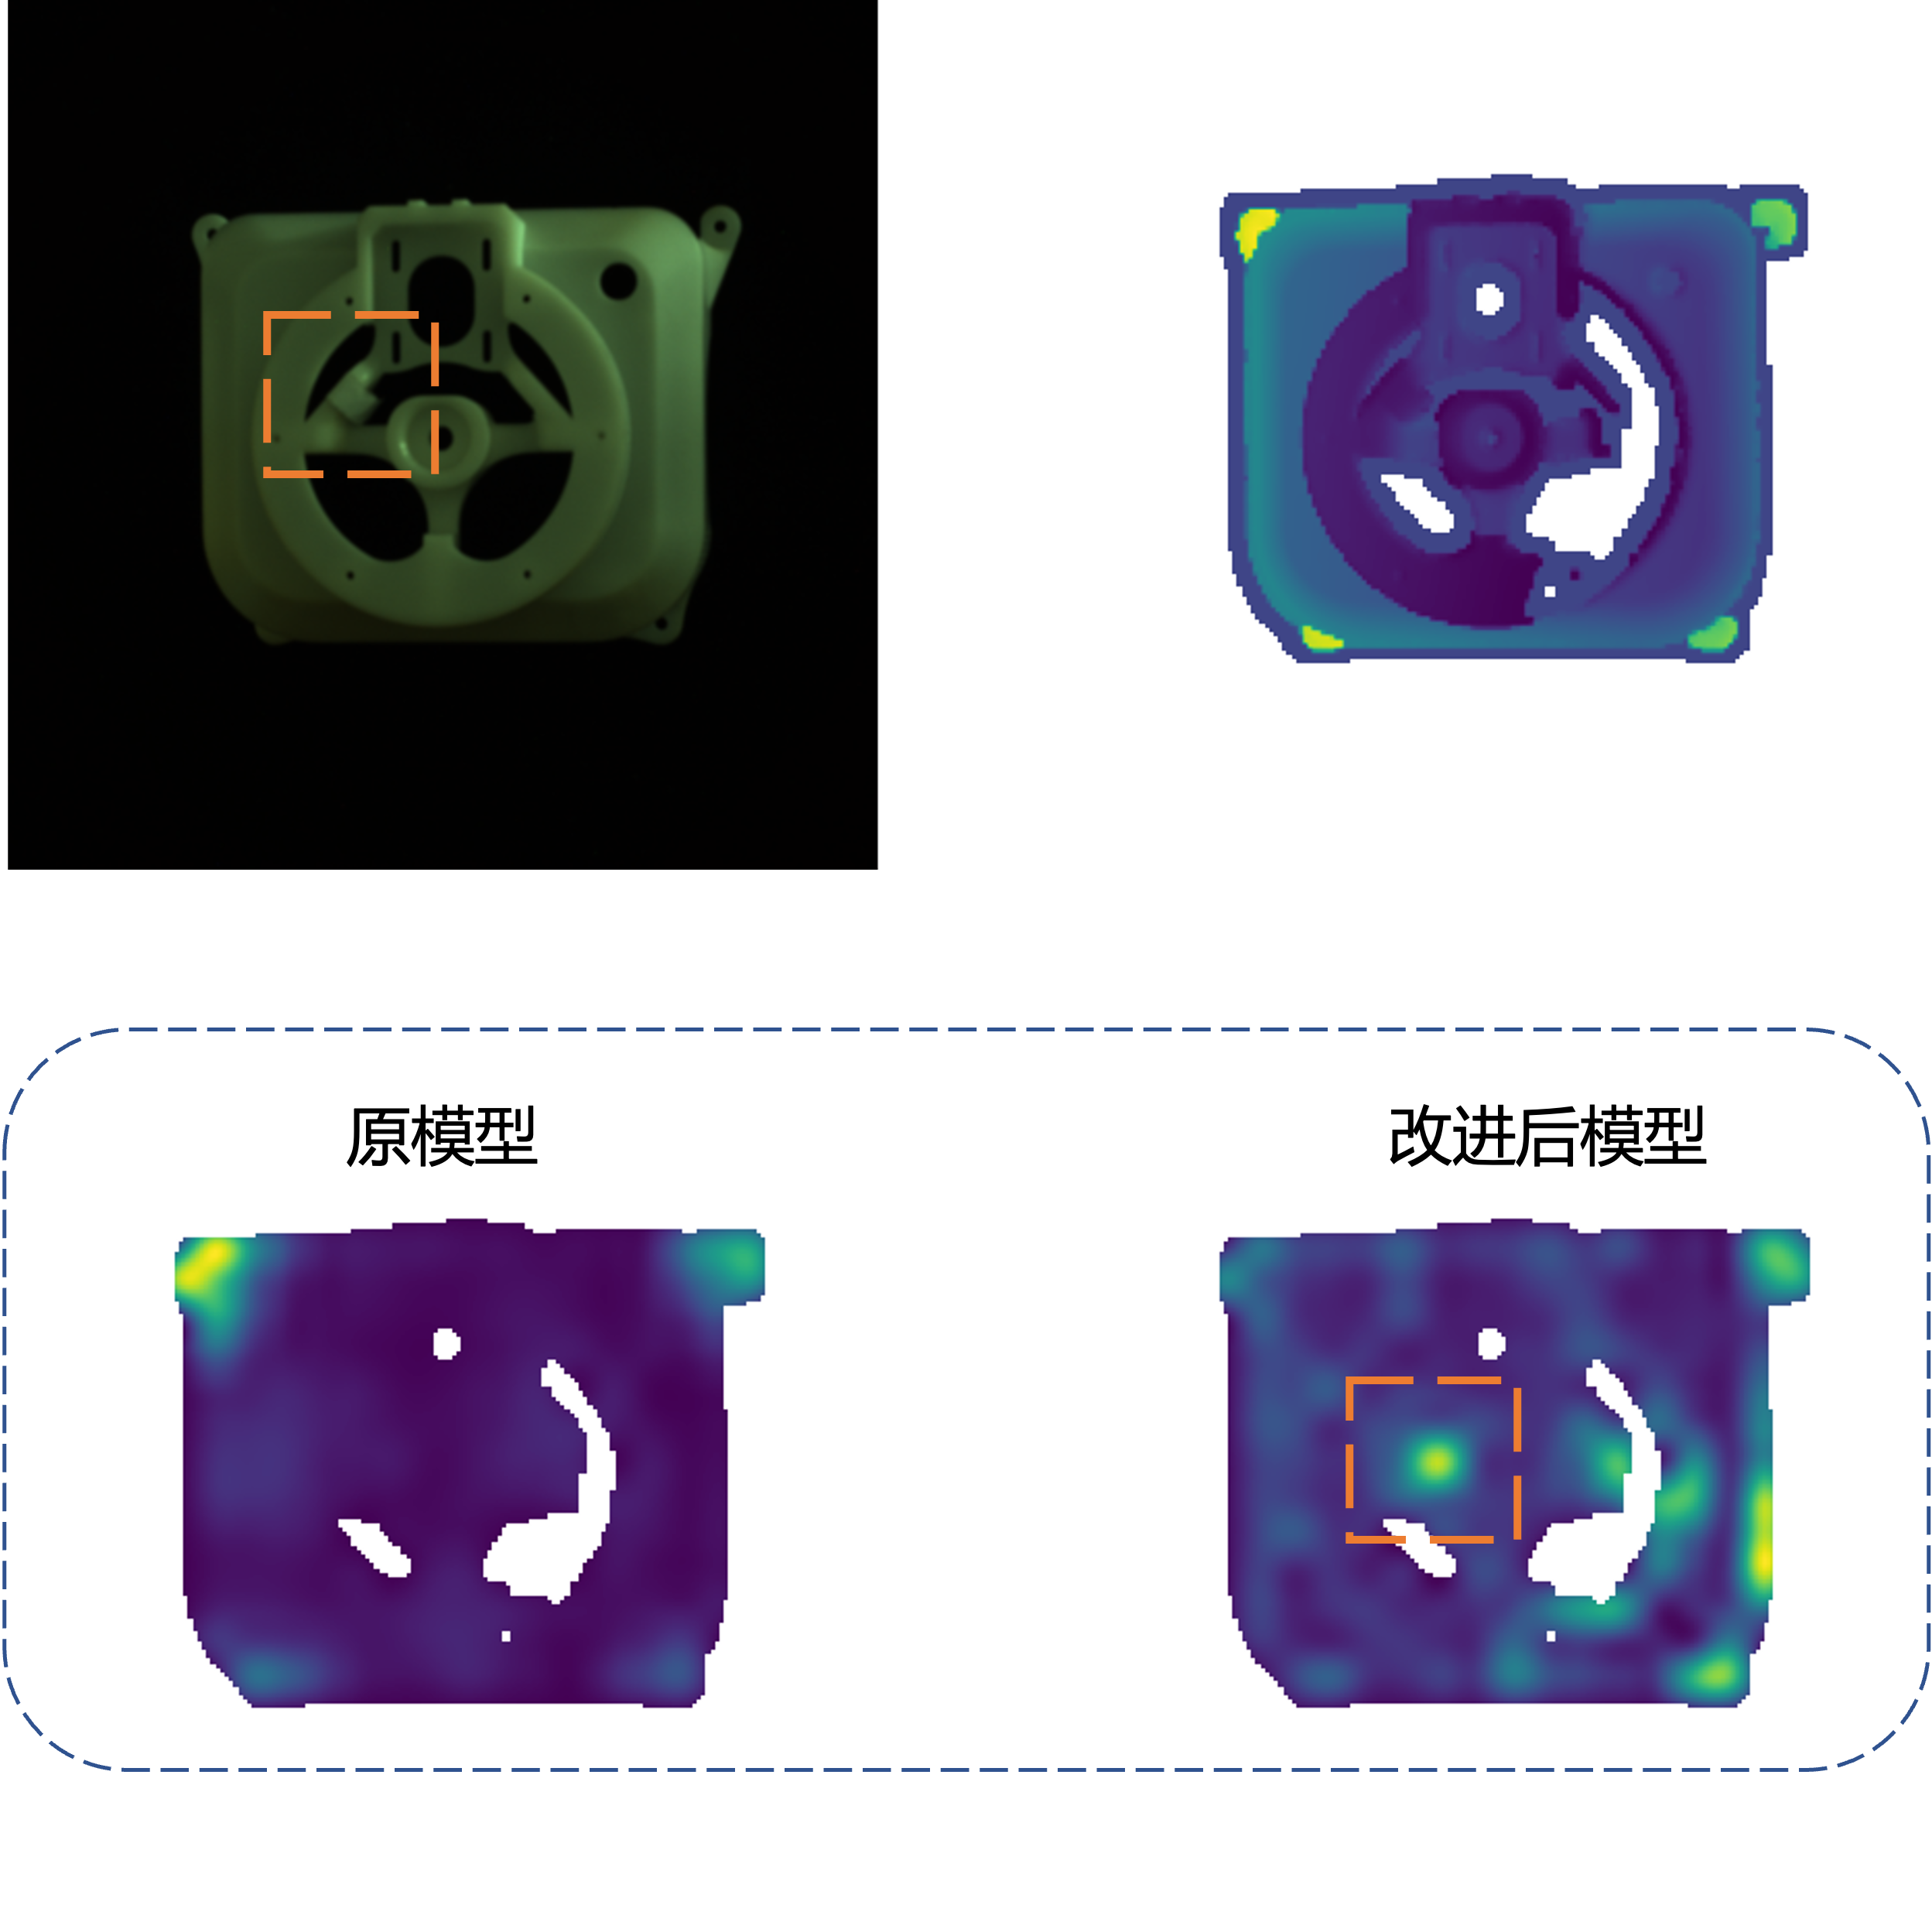
\includegraphics[width=0.6\textwidth]{figures/4/featmap-2.png}
    \caption{结构变型热力图}
    \label{fig:featmap-2}
\end{figure}


\section{本章小节}
本章首先对采集的多模态数据——RGB和深度图像进行预处理,然后分别通过预训练的EfficientNet网络对RGB图像提取特征图和迁移HOG特征描述子到深度图像来提取深度特征,接着分别介绍了本章缺陷检测骨干网络中的标准化流的教师网络和本文改进深度特征融合的学生网络原理。在本章最后的实验阶段,对比了引入HOG提取深度特征和改进学生网络对缺陷算法性能提升,证明了本文提出方法的有效性。

















% \begin{algorithm}
%     \caption{Depth Image Normalization 深度图像归一化}
%     \begin{algorithmic}[1]
%     \Function{NormalizeDepthImage}{$depth\_image$}
%         \State $depth\_image\_float \gets \Call{ConvertToFloat}{depth\_image}$  \Comment{转换为浮点数格式}
%         \State $depth\_image\_float \gets \Call{ReplaceInvalidValues}{depth\_image\_float}$  \Comment{去除无效值}
%         \State $min\_depth, max\_depth \gets \Call{FindMinAndMax}{depth\_image\_float}$  \Comment{计算最小值和最大值}
%         \State $normalized\_depth\_image \gets (depth\_image\_float - min\_depth) / (max\_depth - min\_depth)$  \Comment{归一化处理}
%         \State $normalized\_depth\_image \gets \Call{Denoise}{normalized\_depth\_image}$  \Comment{(可选)去除噪声}
%         \State \Return $normalized\_depth\_image$
%     \EndFunction
    
%     \Function{ConvertToFloat}{$image$}
%         \State \Return $image.astype(float)$  \Comment{将图像转换为浮点数格式}
%     \EndFunction
    
%     \Function{ReplaceInvalidValues}{$image$}
%         \State $image[image \leq 0] \gets 0$  \Comment{将无效值(如NaN或负数)替换为零}
%         \State \Return $image$
%     \EndFunction
    
%     \Function{FindMinAndMax}{$image$}
%         \State $min\_value \gets image[image > 0].min()$  \Comment{找到有效像素值的最小值}
%         \State $max\_value \gets image[image > 0].max()$  \Comment{找到有效像素值的最大值}
%         \State \Return $min\_value, max\_value$
%     \EndFunction
    
%     \Function{Denoise}{$image$}
%         \State $denoised\_image \gets \Call{apply\_denoising\_filter}{image}$  \Comment{使用平滑滤波器(如高斯滤波器或中值滤波器)去除噪声}
%         \State \Return $denoised\_image$
%     \EndFunction
%     \end{algorithmic}
%     \end{algorithm}


    